\begin{small}
\begin{verbatim}
% LaTeX (version 2e) source for "LaTeX for Thesis and Large Documents"
% By Stephen Carr and Wail Gueaieb
% Updated 2005-04-07
%
% Parts to edit are marked by the following block:
%###################################
%## Edit this part
%###################################
% 
% Do NOT edit anything else unless you know what you are doing.
%
%======================================================================
%   P R E A M B L E
%======================================================================
\documentclass[%
12pt,   % font size
oneside,  % final version of thesis has to be submitted single-sided
%twoside, % in case you want to print a draft on both sides of the page
]{report} 
%----------------------------------------------------------------------
%###################################
%## Edit this part
%###################################
\newcommand{\thesisauthor}{Stephen M. Carr and Wail Gueaieb}
\newcommand{\thesistitlecoverpage}{%
  \LaTeX \\ 
  for Thesis \\
  and Large Documents
}
\newcommand{\thesistitleheadings}{\LaTeX for Thesis and Large Documents}
\newcommand{\degree}{Ph.D.} % possible values are:
                          % M.A. / M.A.Sc. / M.Sc. / MCS / Ph.D.
\newcommand{\nameofprogram}{Electrical and Computer Engineering}
\newcommand{\academicunit}{School of Information Technology and Engineering}
\newcommand{\faculty}{Faculty of Engineering}
\newcommand{\graduationyear}{2005}

\newcommand{\abstractfile}{abstract.tex}
\newcommand{\acknowledgementfile}{acknowledgement.tex}
%----------------------------------------------------------------------
% Reprocess only those files which have changed recently:
% \includeonly{intro,creating,commands} 
%----------------------------------------------------------------------
% Create a listing in the log of all files needed to process this document
\listfiles
%----------------------------------------------------------------------
\makeindex % activate index-making
%----------------------------------------------------------------------
% THESIS PREAMBLE
% By Stephen Carr and Wail Gueaieb
% Updated 2005-04-07

% The following command sets "1.2" as the line spacing throughout the
% thesis for readability (optional).
\renewcommand{\baselinestretch}{1.2}
%----------------------------------------------------------------------
% Reset page margins properly for doublesided pages
\usepackage[letterpaper,includehead,left=3.25cm,right=2.5cm,top=2.5cm,headsep=1.5cm,headheight=0.0cm,bottom=2.5cm,footskip=1.0cm]{geometry} 
% \setlength{\marginparwidth}{0pt}
% \setlength{\marginparsep}{0pt}
% \setlength{\oddsidemargin}{0.125in}
% \setlength{\evensidemargin}{0.125in}
% \setlength{\textwidth}{6.375in}
\raggedbottom
%----------------------------------------------------------------------
%%%%%%%%%%%%%%%%%%%%%%%%%%%%%%%%%%%%%%%%%%%%%%%%%%%%%%%%%%%%%
 % thesis-specific settings
%----------------------------------------------------------------------
% My own command and environment definitions:
\newcommand{\program}[1]{\textbf{#1}} % program names in bold text
\newcommand{\exten}[1]{\texttt{#1}} % file extensions in bold text (use caps)
\newcommand{\cmmd}[1]{\textbackslash\texttt{#1}} % command name in tt font 
\newcommand{\enviro}[1]{\texttt{#1}} % environment name in tt font

\newcommand{\eg}{\textit{e.g.},} % some Latin abreviations in italic
\newcommand{\ie}{\textit{i.e.},}
\newcommand{\etc}{\textit{etc}.\@}

\newcommand{\mat}[1]{\ensuremath{\mathcal{#1}}} 
	% matrix names in uppercase caligraphic
\newcommand{\vect}[1]{\ensuremath{\mathit{#1}}} 
% vector names in math italic
\newcommand{\rv}[1]{\ensuremath{\mathbf{#1}}} 
% math bold for random variables
\newcommand{\degg}[1]{\mbox{\raisebox{3pt}{$\circ$}\hspace{-.5pt}#1}}
% command to produce a degree sign. Example: \degg[C] gives degrees Celcius

\newenvironment{definition}[1]{\begin{quote}\emph{#1}:}{\end{quote}}
  % Provides indented formal definition and emphasizes the word.
  % e.g. \begin{definition}{Reliability} ... \end{definition}

\newenvironment{where}[1]% Equation symbol lists
 {\begin{list}{}%
  {\renewcommand{\makelabel}[1]{\hfill\textnormal{##1 =}}%
   \settowidth{\labelwidth}{\textnormal{#1 =}}%
   \setlength{\leftmargin}{\labelwidth}%
   \addtolength{\leftmargin}{\labelsep}%
   \setlength{\itemsep}{-\parsep}}}%
 {\end{list}}
% Example:
% \begin{where}{where $E$}
%  \item[where $E$] least squares error term;
%  \item[$w$] weighting factor associated with each measured variable.
% \end{where}
%----------------------------------------------------------------------
% Standard LaTeX2e packages I am using (as seen in "The LaTeX Companion"):
\usepackage[dvips]{graphicx} 
	% ... if you want to include encapsulated postscript figures
\usepackage{makeidx} % ... if you want an index
\usepackage{amsmath} % ... if you need lots of math symbols
\usepackage[dvips=true,bookmarks=true]{hyperref} 
	% ... only needed for PDF generation
%----------------------------------------------------------------------
% Non-standard packages I am using (things I've written, borrowed, etc.):
%\usepackage{} % ... note that old .sty files can be included here

%======================================================================
%   L O G I C A L    D O C U M E N T
%======================================================================
\begin{document}
%----------------------------------------------------------------------
% FRONT MATERIAL
%----------------------------------------------------------------------
% TITLE PAGE 
% By Stephen Carr and Wail Gueaieb
% Updated 2005-04-07

\pagestyle{empty} % No headers or page numbers

\begin{center}

\vspace*{1.0cm}
{\bf \LARGE %
  \thesistitlecoverpage}

\vspace*{1.0cm}
\normalsize
by \\
\vspace*{1.0cm}
\Large
\thesisauthor\\
\vspace*{2.0cm}
\normalsize
Thesis submitted to the\\
Faculty of Graduate and Postdoctoral Studies\\
In partial fulfillment of the requirements\\
For the \degree~degree in\\
\nameofprogram\\

\vspace*{2.0cm}
\academicunit\\
\faculty\\
University of Ottawa\\

\vspace*{2.0cm}
\copyright~\thesisauthor, Ottawa, Canada, \graduationyear\\

\end{center}

\newpage
 
%%%%%%%%%%%%%%%%%%%%%%%%%%%%%%%%%%%%%%%%%%%%%%%%%%%%%%%%%%%%%

% PRELIMINARY PAGES
\pagestyle{plain} % No headers, just page numbers
\pagenumbering{roman} % Roman numerals
\setcounter{page}{2}

%----------------------------------------------------------------------
% This page is not needed for the University of Ottawa
% % Declaration Page
% \noindent
% I hereby declare that I am the sole author of this thesis.

% \noindent
% I authorize the University of Ottawa to lend this thesis to other
% institutions or individuals for the purpose of scholarly research.
% \vspace{4cm}

% \noindent
% \thesisauthor

% \vspace{4cm}

% \noindent
% I further authorize the University of Ottawa to reproduce this thesis by
% photocopying or other means, in total or in part, at the request of other
% institutions or individuals for the purpose of scholarly research.
% \vspace{4cm}

% \noindent
% \thesisauthor
% \newpage
%----------------------------------------------------------------------

% Long abstract (manually formatted)
\begin{center}
\Large
\textbf{Abstract}
\end{center}
\input{\abstractfile}
\newpage

% Acknowledgements and/or Dedication Pages
\begin{center}\textbf{Acknowledgements}\end{center}
\input{\acknowledgementfile}
\newpage

% Pages which are generated automatically
\setcounter{page}{6} % Set this counter to get correct page numbers
\tableofcontents
\listoftables
\listoffigures
\newpage

% Change page numbering back to Arabic numerals
\pagenumbering{arabic}
%%%%%%%%%%%%%%%%%%%%%%%%%%%%%%%%%%%%%%%%%%%%%%%%%%%%%%%%%%%%%
 
% Title page, declaration, borrowers' page, abstract, acknowlegements, 
% dedication, table of contents, list of tables, list of figures

%----------------------------------------------------------------------
% MAIN BODY
%----------------------------------------------------------------------
% HEADINGS 
% By Stephen Carr and Wail Gueaieb
% Updated 2005-04-07

% Put the document title and page numbers in the header
%\pagestyle{headings}
\pagestyle{myheadings}
% Put title on left & chapter heading goes on right by default
\markboth{\thesistitleheadings}
% Go to normal sized type
\normalsize


 % Specify thesis headings
%----------------------------------------------------------------------
%###################################
%## Edit this part
%###################################
% Chapters 
% Include your "sub" source files here (must have extension .tex)
\chapter{Introduction}
\markright{Introduction} % new right header
%======================================================================
\section{What is \LaTeX ?}
%======================================================================
\LaTeX\index{\LaTeX} is a program for formatting or ``typesetting'' documents. 
Actually, when we talk about \LaTeX\, we are usually referring not only to the 
\program{latex} program, but also to a suite of other utility programs which 
work together to format large, complicated documents or books.

\LaTeX\ is unlike common word processing programs found on micro computers.
It is more like a programming language.
``Source'' files are prepared with a text editor which are then processed by the \program{latex} program to produce the final document.
Tags in the source file tell the \program{latex} program how to format the document.
Also, like a programming language, you can (and should) create your own formatting tags, which are included at the beginning of your source file.

\LaTeX\ is a set of macros written by Leslie Lamport \cite{lamport.book} in the \TeX\ language developed by Donald Knuth \cite{knuth.book}.
You may encounter two versions of \LaTeX .
The ``old'' version is 2.09.
In 1993, a newer version, \LaTeXe , was developed to standardize the many extensions which have been developed to improve functionality.
To distinguish between versions, in \LaTeXe\  the first command in a source document was changed from 
\verb=\documentstyle= 
% \verb command is unusual: delimited by any 2 characters; formatted in-line
to 
\verb=\documentclass=
, and the extension ``packages'' are handled differently (with the new 
\verb=\usepackage=
command).
The standardized packages in \LaTeXe\  are described in a handy companion volume \cite{goossens.book} to Lamport's ``\LaTeX\ Book''\cite{lamport.book}.
These last two books are required reading for serious \LaTeX ing, although often an example document (such as this one) is equally valuable.
%======================================================================
\section{Why Use \LaTeX ?}
%======================================================================
Why use \LaTeX\ rather than a word processing package?
\begin{itemize}
\item The source document is plain (ASCII) text, so is very portable.
Any editor or word processor on any computer can be used to write the source document.
\item \LaTeX\ is available on most computing platforms (the source code is free).
\item It is used by many (especially scientific) publishers to format journals and books.
\item \LaTeX\ takes care of most of the formatting of the document with standard environments based on good typesetting form, letting the author concentrate on the \emph{content}.
\item It is flexible enough to be modified to suit any special needs.
\item \LaTeX\ \emph{easily} keeps track of the numbering and organization of structures in large documents, allowing easy modifications.
\item Large documents can be developed in modular form (chapters or sections in separate files).
\item \LaTeX\ has a superior mathematics formating language with every conceivable mathematical symbol.
\end{itemize}
%======================================================================
\section{Possible Reasons Not To Use \LaTeX}
%======================================================================

\begin{itemize}
\item The software is free --- but you \emph{need} the reference books.
\item There is little on-line help --- although the Web has some information.
\item Error messages can be cryptic, and errors difficult to isolate.
\item You need to constantly be \program{latex}-ing and viewing your source to see what you've done.
\item Word processors, such as WordPerfect, now do a reasonable job of handling large documents (but they're still not as good as \LaTeX ).
\end{itemize}
%======================================================================
\section{Where to Find \LaTeX ?}
%======================================================================
\LaTeX\index{\LaTeX!availability} is available on all Unix hosts on campus.
Since the source is freeware, implementations have been developed for just
about all computing platforms. Some versions are commercial because they provide
additional user interface features such as editors which process the document
in the background, or graphical equation editors. One such commercial product,
Scientific Workplace, is supported at UW\@. It provides a graphical front end to \LaTeX\ in which the user is shielded from the language syntax. See
\texttt{http://ist.uwaterloo.ca/ew/software/scientific/} for details.

\LaTeX\ is not currently on the Waterloo Polaris network.

Also, the Comprehensive TeX Archive Network (CTAN) on the Internet, contains all
 source files and utilities for \LaTeX\ if you wish to download a copy for your
home computer.
 %"What is LaTeX, Why Use It, and Where to Find It?"
\chapter{Creating Your Source File}
\markright{Creating Your Source File} % new right header
%======================================================================
\section{Description of Source File(s)}
%======================================================================
\LaTeX\ source files are just ASCII text files containing the text of your document and the \LaTeX\ mark-up tags.

The mark-up tags are of two types, \emph{commands} and \emph{environments}.
\begin{description}
\item[Command] A command is a single \LaTeX\ tag which performs a specific action, such as inserting some blank space, or toggles a formatting mode on or off, such as a larger type face.
\item[Environment] An environment is a formatting mode which is delimited by \cmmd{begin} and \cmmd{end} statements.
For example, the \enviro{description} environment formats the display of a description offset from the surrounding text. 
Most commands also have an equivalent environment form.
\end{description}
%======================================================================
\section{Organizing Your Source File}
%======================================================================
Some general notes about organization:
\begin{itemize}
\item Clearly denote and comment the sections of your source file.
\item In the main body, put each sentence on a new line, and let the lines wrap.
This makes it easier to edit and move sentences around.
\item Plan your document ahead of time.
Think about what nomenclature you will use.
What \emph{logical structures} are suggested by the nomenclature? 
\item Will you need a bibliography? Do you have a lot of references which you will use again sometime?
\item Will you need an index? If so, plan concepts and words to index.
\end{itemize}
\LaTeX\ can easily keep track of all of these things, but it's easier to create your document if your are thinking about index items, citations and cross-references as you go, rather than as an afterthought! 
%======================================================================
\section{Editing Your Source File}
%======================================================================
Use your favourite text editor.
\begin{itemize}
\item Unix: \program{vi}, \program{emacs}, or the easy \program{pico}
\item PC or Mac: use any editor or word processor (and save as text)
\end{itemize}
Break your document up into several source files, a ``master'' file, and ``subdocuments'' (\eg\ one for each chapter and appendix).
%======================================================================
\section{Parts of the Master Source File}
%======================================================================
\subsection{Preamble}
%----------------------------------------------------------------------
The ``preamble'' of the source file tells the \program{latex} program how to format the structures and commands it finds in your document.

The basic format of the document is provided by the first preamble command, the \cmmd{documentclass} command.
Document classes built-in to \LaTeX\ are \textbf{letter, article, report, book,} and \textbf{slides}.
% - - - - - - - - - - - - - - - - - - - - - - - - - - - - - - - - - - -
\subsubsection{Examples of the \cmmd{documentclass} Command}
% - - - - - - - - - - - - - - - - - - - - - - - - - - - - - - - - - - -
% the \verbatim environment displays the text (i.e. not in-line)
\begin{verbatim}
\documentclass[12pt,2col]{article}
\documentclass[10pt]{report}
\end{verbatim}
Options to this command (and other \LaTeX\ commands) are given in square brackets just before the curly braces.
Options are used to adjust the default point size of text, or other characteristics defined by a class.

UW has added its own modifications to some classes, notably, the \textbf{thesis91e} class.
However, this class uses a several ``styles'' dating from \LaTeX 2.09, which are not now available on many Unix hosts.  
Since all \textbf{thesis91e} does is prepare the front material for the thesis,
which is easily done ``by hand'', it is not necessary.
This document was prepared with the standard \textbf{report} document class.

The formatting commands may be built-in, defined in the standard packages, or defined by the user in the preamble itself with \cmmd{newcommand}. 
The \cmmd{usepackage} command identifies standard \LaTeXe\ packages as well as non-standard 
\footnote{
Note that all packages and options are plain (ASCII) text files written in \LaTeX\ or \TeX , which can be copied and modified by the user.
If you create your own packages or classes, \LaTeX\ will find them if you put them in the same directory as your document source files (or, under Unix, set \program{latex}'s path variables to find them).
} % end footnote
packages (which you could write yourself).
Don't forget to provide non-standard packages along with the other \LaTeX\ source documents if you give them to someone else!
%----------------------------------------------------------------------
\subsection{The Logical Document}
%----------------------------------------------------------------------
The logical document resides inside the \enviro{document} environment.
The document consists, usually, of three parts:
\begin{enumerate}
\item Front material --- title page, table of contents, list of figures, \etc
\item Main body of text --- chapters, sections, subsections, \etc
\item End material --- appendices, bibliography, index
\end{enumerate}
The outline of the logical document should be clear in the master source file.
Use the \cmmd{include} command, \eg\ 
\verb=\include{chap1}=, to include source subdocument \texttt{chap1.tex}.
% - - - - - - - - - - - - - - - - - - - - - - - - - - - - - - - - - - -
\subsubsection{Example Master Source File}
% - - - - - - - - - - - - - - - - - - - - - - - - - - - - - - - - - - -
\label{ex.master}
% paste in course.tex here
\begin{small}
\begin{verbatim}
% LaTeX (version 2e) source for "LaTeX for Thesis and Large Documents"
% By Stephen Carr and Wail Gueaieb
% Updated 2005-04-07
%
% Parts to edit are marked by the following block:
%###################################
%## Edit this part
%###################################
% 
% Do NOT edit anything else unless you know what you are doing.
%
%======================================================================
%   P R E A M B L E
%======================================================================
\documentclass[%
12pt,   % font size
oneside,  % final version of thesis has to be submitted single-sided
%twoside, % in case you want to print a draft on both sides of the page
]{report} 
%----------------------------------------------------------------------
%###################################
%## Edit this part
%###################################
\newcommand{\thesisauthor}{Stephen M. Carr and Wail Gueaieb}
\newcommand{\thesistitlecoverpage}{%
  \LaTeX \\ 
  for Thesis \\
  and Large Documents
}
\newcommand{\thesistitleheadings}{\LaTeX for Thesis and Large Documents}
\newcommand{\degree}{Ph.D.} % possible values are:
                          % M.A. / M.A.Sc. / M.Sc. / MCS / Ph.D.
\newcommand{\nameofprogram}{Electrical and Computer Engineering}
\newcommand{\academicunit}{School of Information Technology and Engineering}
\newcommand{\faculty}{Faculty of Engineering}
\newcommand{\graduationyear}{2005}

\newcommand{\abstractfile}{abstract.tex}
\newcommand{\acknowledgementfile}{acknowledgement.tex}
%----------------------------------------------------------------------
% Reprocess only those files which have changed recently:
% \includeonly{intro,creating,commands} 
%----------------------------------------------------------------------
% Create a listing in the log of all files needed to process this document
\listfiles
%----------------------------------------------------------------------
\makeindex % activate index-making
%----------------------------------------------------------------------
% THESIS PREAMBLE
% By Stephen Carr and Wail Gueaieb
% Updated 2005-04-07

% The following command sets "1.2" as the line spacing throughout the
% thesis for readability (optional).
\renewcommand{\baselinestretch}{1.2}
%----------------------------------------------------------------------
% Reset page margins properly for doublesided pages
\usepackage[letterpaper,includehead,left=3.25cm,right=2.5cm,top=2.5cm,headsep=1.5cm,headheight=0.0cm,bottom=2.5cm,footskip=1.0cm]{geometry} 
% \setlength{\marginparwidth}{0pt}
% \setlength{\marginparsep}{0pt}
% \setlength{\oddsidemargin}{0.125in}
% \setlength{\evensidemargin}{0.125in}
% \setlength{\textwidth}{6.375in}
\raggedbottom
%----------------------------------------------------------------------
%%%%%%%%%%%%%%%%%%%%%%%%%%%%%%%%%%%%%%%%%%%%%%%%%%%%%%%%%%%%%
 % thesis-specific settings
%----------------------------------------------------------------------
% My own command and environment definitions:
\newcommand{\program}[1]{\textbf{#1}} % program names in bold text
\newcommand{\exten}[1]{\texttt{#1}} % file extensions in bold text (use caps)
\newcommand{\cmmd}[1]{\textbackslash\texttt{#1}} % command name in tt font 
\newcommand{\enviro}[1]{\texttt{#1}} % environment name in tt font

\newcommand{\eg}{\textit{e.g.},} % some Latin abreviations in italic
\newcommand{\ie}{\textit{i.e.},}
\newcommand{\etc}{\textit{etc}.\@}

\newcommand{\mat}[1]{\ensuremath{\mathcal{#1}}} 
	% matrix names in uppercase caligraphic
\newcommand{\vect}[1]{\ensuremath{\mathit{#1}}} 
% vector names in math italic
\newcommand{\rv}[1]{\ensuremath{\mathbf{#1}}} 
% math bold for random variables
\newcommand{\degg}[1]{\mbox{\raisebox{3pt}{$\circ$}\hspace{-.5pt}#1}}
% command to produce a degree sign. Example: \degg[C] gives degrees Celcius

\newenvironment{definition}[1]{\begin{quote}\emph{#1}:}{\end{quote}}
  % Provides indented formal definition and emphasizes the word.
  % e.g. \begin{definition}{Reliability} ... \end{definition}

\newenvironment{where}[1]% Equation symbol lists
 {\begin{list}{}%
  {\renewcommand{\makelabel}[1]{\hfill\textnormal{##1 =}}%
   \settowidth{\labelwidth}{\textnormal{#1 =}}%
   \setlength{\leftmargin}{\labelwidth}%
   \addtolength{\leftmargin}{\labelsep}%
   \setlength{\itemsep}{-\parsep}}}%
 {\end{list}}
% Example:
% \begin{where}{where $E$}
%  \item[where $E$] least squares error term;
%  \item[$w$] weighting factor associated with each measured variable.
% \end{where}
%----------------------------------------------------------------------
% Standard LaTeX2e packages I am using (as seen in "The LaTeX Companion"):
\usepackage[dvips]{graphicx} 
	% ... if you want to include encapsulated postscript figures
\usepackage{makeidx} % ... if you want an index
\usepackage{amsmath} % ... if you need lots of math symbols
\usepackage[dvips=true,bookmarks=true]{hyperref} 
	% ... only needed for PDF generation
%----------------------------------------------------------------------
% Non-standard packages I am using (things I've written, borrowed, etc.):
%\usepackage{} % ... note that old .sty files can be included here

%======================================================================
%   L O G I C A L    D O C U M E N T
%======================================================================
\begin{document}
%----------------------------------------------------------------------
% FRONT MATERIAL
%----------------------------------------------------------------------
% TITLE PAGE 
% By Stephen Carr and Wail Gueaieb
% Updated 2005-04-07

\pagestyle{empty} % No headers or page numbers

\begin{center}

\vspace*{1.0cm}
{\bf \LARGE %
  \thesistitlecoverpage}

\vspace*{1.0cm}
\normalsize
by \\
\vspace*{1.0cm}
\Large
\thesisauthor\\
\vspace*{2.0cm}
\normalsize
Thesis submitted to the\\
Faculty of Graduate and Postdoctoral Studies\\
In partial fulfillment of the requirements\\
For the \degree~degree in\\
\nameofprogram\\

\vspace*{2.0cm}
\academicunit\\
\faculty\\
University of Ottawa\\

\vspace*{2.0cm}
\copyright~\thesisauthor, Ottawa, Canada, \graduationyear\\

\end{center}

\newpage
 
%%%%%%%%%%%%%%%%%%%%%%%%%%%%%%%%%%%%%%%%%%%%%%%%%%%%%%%%%%%%%

% PRELIMINARY PAGES
\pagestyle{plain} % No headers, just page numbers
\pagenumbering{roman} % Roman numerals
\setcounter{page}{2}

%----------------------------------------------------------------------
% This page is not needed for the University of Ottawa
% % Declaration Page
% \noindent
% I hereby declare that I am the sole author of this thesis.

% \noindent
% I authorize the University of Ottawa to lend this thesis to other
% institutions or individuals for the purpose of scholarly research.
% \vspace{4cm}

% \noindent
% \thesisauthor

% \vspace{4cm}

% \noindent
% I further authorize the University of Ottawa to reproduce this thesis by
% photocopying or other means, in total or in part, at the request of other
% institutions or individuals for the purpose of scholarly research.
% \vspace{4cm}

% \noindent
% \thesisauthor
% \newpage
%----------------------------------------------------------------------

% Long abstract (manually formatted)
\begin{center}
\Large
\textbf{Abstract}
\end{center}
\input{\abstractfile}
\newpage

% Acknowledgements and/or Dedication Pages
\begin{center}\textbf{Acknowledgements}\end{center}
\input{\acknowledgementfile}
\newpage

% Pages which are generated automatically
\setcounter{page}{6} % Set this counter to get correct page numbers
\tableofcontents
\listoftables
\listoffigures
\newpage

% Change page numbering back to Arabic numerals
\pagenumbering{arabic}
%%%%%%%%%%%%%%%%%%%%%%%%%%%%%%%%%%%%%%%%%%%%%%%%%%%%%%%%%%%%%
 
% Title page, declaration, borrowers' page, abstract, acknowlegements, 
% dedication, table of contents, list of tables, list of figures

%----------------------------------------------------------------------
% MAIN BODY
%----------------------------------------------------------------------
% HEADINGS 
% By Stephen Carr and Wail Gueaieb
% Updated 2005-04-07

% Put the document title and page numbers in the header
%\pagestyle{headings}
\pagestyle{myheadings}
% Put title on left & chapter heading goes on right by default
\markboth{\thesistitleheadings}
% Go to normal sized type
\normalsize


 % Specify thesis headings
%----------------------------------------------------------------------
%###################################
%## Edit this part
%###################################
% Chapters 
% Include your "sub" source files here (must have extension .tex)
\chapter{Introduction}
\markright{Introduction} % new right header
%======================================================================
\section{What is \LaTeX ?}
%======================================================================
\LaTeX\index{\LaTeX} is a program for formatting or ``typesetting'' documents. 
Actually, when we talk about \LaTeX\, we are usually referring not only to the 
\program{latex} program, but also to a suite of other utility programs which 
work together to format large, complicated documents or books.

\LaTeX\ is unlike common word processing programs found on micro computers.
It is more like a programming language.
``Source'' files are prepared with a text editor which are then processed by the \program{latex} program to produce the final document.
Tags in the source file tell the \program{latex} program how to format the document.
Also, like a programming language, you can (and should) create your own formatting tags, which are included at the beginning of your source file.

\LaTeX\ is a set of macros written by Leslie Lamport \cite{lamport.book} in the \TeX\ language developed by Donald Knuth \cite{knuth.book}.
You may encounter two versions of \LaTeX .
The ``old'' version is 2.09.
In 1993, a newer version, \LaTeXe , was developed to standardize the many extensions which have been developed to improve functionality.
To distinguish between versions, in \LaTeXe\  the first command in a source document was changed from 
\verb=\documentstyle= 
% \verb command is unusual: delimited by any 2 characters; formatted in-line
to 
\verb=\documentclass=
, and the extension ``packages'' are handled differently (with the new 
\verb=\usepackage=
command).
The standardized packages in \LaTeXe\  are described in a handy companion volume \cite{goossens.book} to Lamport's ``\LaTeX\ Book''\cite{lamport.book}.
These last two books are required reading for serious \LaTeX ing, although often an example document (such as this one) is equally valuable.
%======================================================================
\section{Why Use \LaTeX ?}
%======================================================================
Why use \LaTeX\ rather than a word processing package?
\begin{itemize}
\item The source document is plain (ASCII) text, so is very portable.
Any editor or word processor on any computer can be used to write the source document.
\item \LaTeX\ is available on most computing platforms (the source code is free).
\item It is used by many (especially scientific) publishers to format journals and books.
\item \LaTeX\ takes care of most of the formatting of the document with standard environments based on good typesetting form, letting the author concentrate on the \emph{content}.
\item It is flexible enough to be modified to suit any special needs.
\item \LaTeX\ \emph{easily} keeps track of the numbering and organization of structures in large documents, allowing easy modifications.
\item Large documents can be developed in modular form (chapters or sections in separate files).
\item \LaTeX\ has a superior mathematics formating language with every conceivable mathematical symbol.
\end{itemize}
%======================================================================
\section{Possible Reasons Not To Use \LaTeX}
%======================================================================

\begin{itemize}
\item The software is free --- but you \emph{need} the reference books.
\item There is little on-line help --- although the Web has some information.
\item Error messages can be cryptic, and errors difficult to isolate.
\item You need to constantly be \program{latex}-ing and viewing your source to see what you've done.
\item Word processors, such as WordPerfect, now do a reasonable job of handling large documents (but they're still not as good as \LaTeX ).
\end{itemize}
%======================================================================
\section{Where to Find \LaTeX ?}
%======================================================================
\LaTeX\index{\LaTeX!availability} is available on all Unix hosts on campus.
Since the source is freeware, implementations have been developed for just
about all computing platforms. Some versions are commercial because they provide
additional user interface features such as editors which process the document
in the background, or graphical equation editors. One such commercial product,
Scientific Workplace, is supported at UW\@. It provides a graphical front end to \LaTeX\ in which the user is shielded from the language syntax. See
\texttt{http://ist.uwaterloo.ca/ew/software/scientific/} for details.

\LaTeX\ is not currently on the Waterloo Polaris network.

Also, the Comprehensive TeX Archive Network (CTAN) on the Internet, contains all
 source files and utilities for \LaTeX\ if you wish to download a copy for your
home computer.
 %"What is LaTeX, Why Use It, and Where to Find It?"
\chapter{Creating Your Source File}
\markright{Creating Your Source File} % new right header
%======================================================================
\section{Description of Source File(s)}
%======================================================================
\LaTeX\ source files are just ASCII text files containing the text of your document and the \LaTeX\ mark-up tags.

The mark-up tags are of two types, \emph{commands} and \emph{environments}.
\begin{description}
\item[Command] A command is a single \LaTeX\ tag which performs a specific action, such as inserting some blank space, or toggles a formatting mode on or off, such as a larger type face.
\item[Environment] An environment is a formatting mode which is delimited by \cmmd{begin} and \cmmd{end} statements.
For example, the \enviro{description} environment formats the display of a description offset from the surrounding text. 
Most commands also have an equivalent environment form.
\end{description}
%======================================================================
\section{Organizing Your Source File}
%======================================================================
Some general notes about organization:
\begin{itemize}
\item Clearly denote and comment the sections of your source file.
\item In the main body, put each sentence on a new line, and let the lines wrap.
This makes it easier to edit and move sentences around.
\item Plan your document ahead of time.
Think about what nomenclature you will use.
What \emph{logical structures} are suggested by the nomenclature? 
\item Will you need a bibliography? Do you have a lot of references which you will use again sometime?
\item Will you need an index? If so, plan concepts and words to index.
\end{itemize}
\LaTeX\ can easily keep track of all of these things, but it's easier to create your document if your are thinking about index items, citations and cross-references as you go, rather than as an afterthought! 
%======================================================================
\section{Editing Your Source File}
%======================================================================
Use your favourite text editor.
\begin{itemize}
\item Unix: \program{vi}, \program{emacs}, or the easy \program{pico}
\item PC or Mac: use any editor or word processor (and save as text)
\end{itemize}
Break your document up into several source files, a ``master'' file, and ``subdocuments'' (\eg\ one for each chapter and appendix).
%======================================================================
\section{Parts of the Master Source File}
%======================================================================
\subsection{Preamble}
%----------------------------------------------------------------------
The ``preamble'' of the source file tells the \program{latex} program how to format the structures and commands it finds in your document.

The basic format of the document is provided by the first preamble command, the \cmmd{documentclass} command.
Document classes built-in to \LaTeX\ are \textbf{letter, article, report, book,} and \textbf{slides}.
% - - - - - - - - - - - - - - - - - - - - - - - - - - - - - - - - - - -
\subsubsection{Examples of the \cmmd{documentclass} Command}
% - - - - - - - - - - - - - - - - - - - - - - - - - - - - - - - - - - -
% the \verbatim environment displays the text (i.e. not in-line)
\begin{verbatim}
\documentclass[12pt,2col]{article}
\documentclass[10pt]{report}
\end{verbatim}
Options to this command (and other \LaTeX\ commands) are given in square brackets just before the curly braces.
Options are used to adjust the default point size of text, or other characteristics defined by a class.

UW has added its own modifications to some classes, notably, the \textbf{thesis91e} class.
However, this class uses a several ``styles'' dating from \LaTeX 2.09, which are not now available on many Unix hosts.  
Since all \textbf{thesis91e} does is prepare the front material for the thesis,
which is easily done ``by hand'', it is not necessary.
This document was prepared with the standard \textbf{report} document class.

The formatting commands may be built-in, defined in the standard packages, or defined by the user in the preamble itself with \cmmd{newcommand}. 
The \cmmd{usepackage} command identifies standard \LaTeXe\ packages as well as non-standard 
\footnote{
Note that all packages and options are plain (ASCII) text files written in \LaTeX\ or \TeX , which can be copied and modified by the user.
If you create your own packages or classes, \LaTeX\ will find them if you put them in the same directory as your document source files (or, under Unix, set \program{latex}'s path variables to find them).
} % end footnote
packages (which you could write yourself).
Don't forget to provide non-standard packages along with the other \LaTeX\ source documents if you give them to someone else!
%----------------------------------------------------------------------
\subsection{The Logical Document}
%----------------------------------------------------------------------
The logical document resides inside the \enviro{document} environment.
The document consists, usually, of three parts:
\begin{enumerate}
\item Front material --- title page, table of contents, list of figures, \etc
\item Main body of text --- chapters, sections, subsections, \etc
\item End material --- appendices, bibliography, index
\end{enumerate}
The outline of the logical document should be clear in the master source file.
Use the \cmmd{include} command, \eg\ 
\verb=\include{chap1}=, to include source subdocument \texttt{chap1.tex}.
% - - - - - - - - - - - - - - - - - - - - - - - - - - - - - - - - - - -
\subsubsection{Example Master Source File}
% - - - - - - - - - - - - - - - - - - - - - - - - - - - - - - - - - - -
\label{ex.master}
% paste in course.tex here
\input{mastersource}
 %"Creating Your Source File"
%======================================================================
\chapter{Example \LaTeX\ Commands for Typical Large Documents}
\markright{Example \LaTeX\ Commands for Typical Large Documents}
%======================================================================
For details of the many \LaTeX\ commands, the reference books are indispensable.
However, examples of some structures you will likely need are given here.

\LaTeX\ formatting tags include both \emph{commands} and \emph{environments}.
A command is like a switch; it turns a certain mode on until it is changed or ended by the extent of its ``scope'', delimited by curly braces (or by default, such as the end of a paragraph).
Examples of commands are ``\verb=\emph{really} big='' to emphasize a word and ``\verb=\large='' to turn on large text until it is changed again.
An environment has an explicitly defined scope, indicated by \cmmd{begin} and \cmmd{end} commands, \eg \verb=\begin{equation} ... \end{equation}=.
All commands also have an environment form.
See the Glossary of Terms on page~\pageref{chap.glossary} for more key concepts. 
%======================================================================
\section{Selected Text Structures}
%======================================================================
\subsection{Basic In-Line Commands}
%----------------------------------------------------------------------
\begin{itemize}
\item \LaTeX\ ignores    extra   spaces    in the input.
Add space with \verb*=\ =, \ie\ $\backslash$ followed by a space.
\item Separate paragraphs with a blank line.
\item \LaTeX\ ignores anything after a \% character (comment symbol).
\item \emph{Emphasize} text with the \cmmd{emph} command (italicizes).
\item \LaTeX\ recognizes three types of dashes
	\begin{itemize}
	\item Punctuation ( - - - , or \cmmd{textmdash}): He jumped --- but not high enough!
	\item Range ( - - , or \cmmd{textndash}): Read chapters 1--12 for tomorrow's class.
	\item Interword ( - ): What a thought-provoking essay!
	\end{itemize}
\item Use pairs of opening and closing \emph{single} quotes rather than double quotes, to get ``this'' rather than "this".
\item Ellipsis \ldots\ is produced with the \cmmd{ldots} command.
\item Produce some of \LaTeX 's special symbols with a backslash preceding them \eg\ produce \$, \&, \%, \#, \_, \{ and  \} with \cmmd{\$}, \etc .
\item Produce the remaining special characters \verb=\=, \verb=~=, and \verb=^=, with the \cmmd{verb} command or inside a \enviro{verbatim} environment, or use text mode commands: \cmmd{textbackslash}, \cmmd{textasciitilde}, \cmmd{textasciicircum}, respectively.
\item If you end a sentence with an upper case letter, let \LaTeX\ know with a \cmmd{@} before the closing punctuation, \eg\ \verb=Jane works for ABC\@?=
\item Prevent inappropriate line breaks with a \verb=~= \eg\ \verb=Ms.~Wong=
\item Special accented characters may also be produced, \eg\ \verb=\"{o}= creates \"{o}.
Many other special symbols can be produced in math mode.
\end{itemize}
%----------------------------------------------------------------------
\subsection{Chapters, Sections and Subsections}
%----------------------------------------------------------------------
Logical structures of a document are preceded by commands.
\begin{verbatim}
\chapter{A Chapter Heading}
\section{A Section Heading}
A sentence.
%
\subsection{A Subsection Heading}
A sentence.
\subsubsection{A Subsubsection Heading}
A sentence.
\end{verbatim}
\LaTeX\ takes care of numbering these structures.

\subsubsection{Long Headings and the Table of Contents}
It is often the case that long chapter, section or caption names should be
formatted differently in the Table of Contents than in the body of your thesis.
The way to achieve this is to use an option field in the chapter, section, caption tag to contain the form of the heading that should appear in the Table of Contents, \eg :
\begin{verbatim}
\chapter[Introduction]{Introduction: Motivation for My Research}
\end{verbatim}
Here, the Table of Contents will use the shorter chapter title, and the longer
one will appear as the actual chapter title. This is also a handy method to use
if you want the actual chapter title to contain a line break command (\textbackslash\textbackslash) while that's not necessary in the Table of Contents because of the smaller font used.

\subsubsection{Unnumbered sections}
There is a way to suppress the automatic numbering of several kinds of document
structures. This is achieved by using the ``star'' form of the \LaTeX\ command.
For example to suppress the numbering of a paticular section:
\begin{verbatim}
\section*{A Section With No Number}
\end{verbatim}
The starred form also exists for other automatically numbered document structures such as equations. 
%----------------------------------------------------------------------
\subsection{Displayed Text Structures}
%----------------------------------------------------------------------
There are many structures for displaying text.
Here are some examples:
% - - - - - - - - - - - - - - - - - - - - - - - - - - - - - - - - - - - 
\subsubsection{Lists}
% - - - - - - - - - - - - - - - - - - - - - - - - - - - - - - - - - - -
For un-numbered lists use the \enviro{itemize} environment.
For example,
\begin{verbatim}
   \begin{itemize}
   \item Birds
      \begin{itemize}
      \item ducks
      \item sparrows
      \end{itemize}
   \item Mammals
      \begin{itemize}
      \item dogs
      \item whales
      \end{itemize}
   \end{itemize}
\end{verbatim}
produces
   \begin{itemize}
   \item Birds
      \begin{itemize}
      \item ducks
      \item sparrows
      \end{itemize}
   \item Mammals
      \begin{itemize}
      \item dogs
      \item whales
      \end{itemize}
   \end{itemize}
For numbered lists use the \enviro{enumerate} environment.

For definitions or descriptions use the \enviro{description} environment (see Appendix~\ref{chap.glossary}).
\begin{verbatim}
   \begin{description}
   \item[Dog] Humankind's best friend.
   \end{description}
\end{verbatim}
\begin{description}
\item[Dog] Humankind's best friend.
\end{description}
% - - - - - - - - - - - - - - - - - - - - - - - - - - - - - - - - - - -
\subsubsection{Quotations}
% - - - - - - - - - - - - - - - - - - - - - - - - - - - - - - - - - - -
Use the \enviro{quote} environment for short quotes.
\begin{verbatim}
   \begin{quote}
   If, at first, you don't succeed, try, try again. \emph{Anonymous}
   \end{quote}
\end{verbatim}
\begin{quote}
   If, at first, you don't succeed, try, try again. \emph{Anonymous}
\end{quote}
Use the \enviro{quotation} environment for quotations containing more than
 one paragraph.
% - - - - - - - - - - - - - - - - - - - - - - - - - - - - - - - - - - -
\subsubsection{Free-Form Text}
% - - - - - - - - - - - - - - - - - - - - - - - - - - - - - - - - - - -
The \enviro{verse} environment can be used to display free-form typeset text.
\begin{verbatim}
   \begin{verse}
   The verse environment lets you\\
   break the lines wherever you like. If you go on too long ...
   \end{verse}
\end{verbatim}
\begin{verse}
The verse environment lets you\\
break the lines wherever you like. If you go on too long, though, the line will eventually get broken for you.
\end{verse}
The \enviro{verbatim} environment allows literal text to be printed.
It uses a monospaced font to preserve spaces in the input and allows all special characters to be printed.
Lines are not broken by \LaTeX.
\begin{verbatim}
   \begin{verbatim}
   @#$%@#     $%%^!@#!
   \en {verbatim}
\end{verbatim}
\begin{verbatim}
@#$%@#     $%%^!@#!
\end{verbatim}

Short pieces of literal text may be inserted in a line with the \cmmd{verb} command.
This command is delimited by any two characters rather than by curly braces, \eg\ \newline ``\verb=\verb+some literal text \\%^+=''.
%======================================================================
\section{Cross-References}
%======================================================================
Cross-references are produced with the \cmmd{label} and \cmmd{ref} commands.
\begin{verbatim}
   \section{Discussion}
   \label{sec.discussion}
   .
   . 
   .
   As discussed in Section~\ref{sec.discussion}, ...
\end{verbatim}
Page references may be generated with the \cmmd{pageref} command.
\begin{verbatim}
   As discussed in Section~\ref{sec.discussion} 
   (page~\pageref{sec.discussion}) ... 
\end{verbatim}
%======================================================================
\section{Text Fonts}
%======================================================================
\LaTeX\ has commands which allow the user to select the font family as well as the shape, weight, and size of the characters.
It is important to know that there are different commands for text mode and math mode.
Math fonts are discussed in Section~\ref{ssec.mathfonts}. 
%----------------------------------------------------------------------
\subsection{Font Selection}
%----------------------------------------------------------------------
The default font used by \LaTeX\ is called Computer Modern, designed by Donald Knuth.
Only recently --- just pre-\LaTeXe\ --- has it been (easily) possible to select other styles of fonts in LaTeX documents.
The default font for the whole document may be selected with the \cmmd{usepackage} command.
%\footnote{Under Unix, look in the directory /software/share/latex2e_psnfss/data/inputs to see what fonts are available, \eg\ bookman.sty.}.
%----------------------------------------------------------------------
\subsection{Font Family, Series, and Shape Selection}
\label{ssec.fontfam}
%----------------------------------------------------------------------
Once the default font family is chosen, \LaTeX\ commands may be employed to change the family, series, and shape characteristics.
It should be emphasized that these changes should usually be defined in structure commands (defined in the preamble), rather than used directly in the text.
Then, if you change your mind about how you want some object or concept identified, you just have to change the definition in the preamble for it to take place everywhere.

The font \emph{family} is one of roman, sans serif, or typewriter (monospaced).
The \emph{series} is defined by weight (boldness) and width and may be either bold or medium.
The \emph{shape} may be upright (the default), italic, slanted, or small capitals.

Text-mode commands for controlling these attributes are:
\begin{tabbing}
mmmmm\=mmmmmmmmmmmmm\= \kill
\>\textbf{Command} \>\textbf{Description} \\
\>\cmmd{textrm} \>\textrm{roman family}\\
\>\cmmd{textsf} \>\textsf{sans serif family}\\
\>\cmmd{texttt} \>\texttt{typewriter family}\\
\>\cmmd{textbf} \>\textbf{bold series}\\
\>\cmmd{textmd} \>\textmd{medium series}\\
\>\cmmd{textit} \>\textit{italic shape}\\
\>\cmmd{textsl} \>\textsl{slanted shape}\\
\>\cmmd{textup} \>\textup{upright shape} (default)
\end{tabbing}
%----------------------------------------------------------------------
\subsection{Text Size}
%----------------------------------------------------------------------
Text size is controlled relative to the default size selected in the \cmmd{documentclass} command.

Size commands include \cmmd{tiny}, \cmmd{small}, \cmmd{large}, \cmmd{Large}, \cmmd{LARGE}, \cmmd{huge}, \cmmd{Huge}, \cmmd{normalsize}, \cmmd{footnotesize}, and produce the following effects: \newline
\tiny{tiny} \small{small} \large{large} \Large{Large} \LARGE{LARGE} \huge{huge} \Huge{Huge} \normalsize{normalsize} \footnotesize{footnotesize} \normalsize
%======================================================================
\section{Figures}
%======================================================================
\LaTeX\ has its own built-in drawing capabilities in the \enviro{picture} environment, which allows the user to draw pictures composed of text, lines, arrows, simple curves, and geometric shapes.
However, it is probably easier to use a drawing package to create your figures, then include them as Encapsulated PostScript (EPS) files.
Whenever possible, save your drawings as EPS files (a form of PS designed for embedded figures), rather than as PostScript (PS), which includes full page formatting information.
If necessary, however, PS files can be converted to EPS by adding the ``bounding box'' co-ordinates to the top of the PS file.

\LaTeX\ allows inclusion of PostScript figures with the \enviro{graphicx} package.
EPS files are simply embedded in the output device-independent (DVI) file for processing by a PostScript post-processor such as \program(dvips).
The \enviro{graphicx} package allows the figure to be sized and rotated as desired.
To achieve legibility, however, it is best to \emph{draw} the figure the size you want it.

Here is an example of an included EPS figure and its \LaTeX\ source code.
Figure~\ref{fig.beam} shows a cantilever beam of circular cross-section
subjected to a point load ($\rv{p}$) and a uniformly distributed load
($\rv{q}$), both of which are uncertain.
The length of the beam, ($\rv{l}$), and its physical properties,
Young's modulus ($\rv{e}$) and ultimate bending stress ($\rv{b}$), are also
fixed but uncertain.
The random inputs of the design problem are then $\rv{V}=[\rv{p}, \;
\rv{q}, \; \rv{l}, \; \rv{e}, \; \rv{b} ]^T$.
\begin{figure}[!htbp]
 \begin{center}
  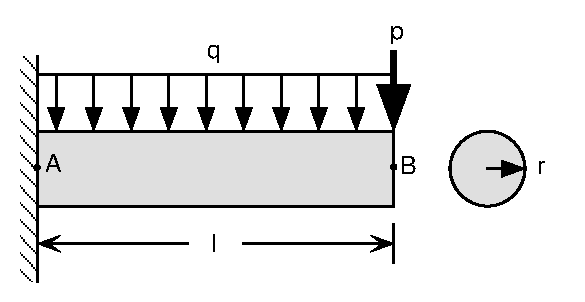
\includegraphics[clip=true]{beam.eps}
 \end{center}
\caption{Cantilever Beam}
\label{fig.beam}
\end{figure}
\begin{verbatim}
\begin{figure}[!htbp]
 \begin{center}
  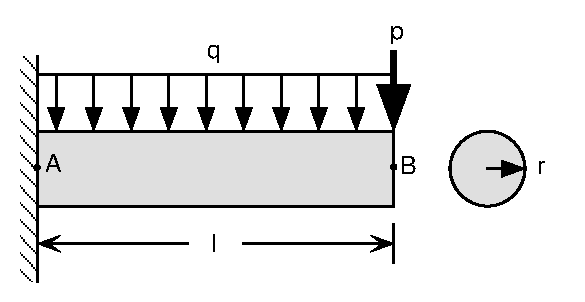
\includegraphics[clip=true]{beam.eps}
 \end{center}
\caption{Cantilever Beam}
\label{fig.beam}
\end{figure}
\end{verbatim}
Note the \enviro{figure} environment, which provides for captioning, and \enviro{center} environment for positioning the figure.

Figures can also be pasted in by hand if you leave room for them.
The following commands will leave a vertical space of 2.5 inches with a caption.
\begin{verbatim}
\begin{figure}
\vspace{2.5in}
\caption{Caption for Figure and for List of Figures - up to 300 chars}
\end{figure}
\end{verbatim}
%======================================================================
\section{Tables}
%======================================================================
Tables are easy to generate in \LaTeX .
Simple tables can be produced with the \enviro{tabbing} environment, as seen
in Section~\ref{ssec.fontfam}.
The source for that table is as follows:
\begin{verbatim}
\begin{tabbing}
mmmmm\=mmmmmmmmmmmmm\= \kill
\>\textbf{Command} \>\textbf{Description} \\
\>\cmmd{textrm} \>roman family \\
\>\cmmd{textsf} \>sans serif family \\
\>\cmmd{texttt} \>typewriter family \\
\>\cmmd{textbf} \>bold series \\
\>\cmmd{textmd} \>medium series \\
\>\cmmd{textit} \>italic shape \\
\>\cmmd{textsl} \>slanted shape \\
\>\cmmd{textup} \>upright shape (default)
\end{tabbing}
\end{verbatim}
Tabs are set with \cmmd{=}.
The \cmmd{kill} command cancels the line after the tabs are set. 
The \cmmd{>} moves to the next set tab stop.

The \enviro{table} and \enviro{tabular} environments can be used to produce captioned and bordered tables.
The following Table~\ref{tab.results} provides an example.
\begin{table}[!htbp]
\begin{center}
\begin{tabular}{|c||cc|cc|}
\hline
& \multicolumn{2}{c|}{ {\textbf CCP Rel. Indices} } 
& \multicolumn{2}{c|}{ {\textbf FORM Rel. Indices} } \\ 
\cline{2-5}
& $\beta_{MVFO}$ & $\beta_{MVMS}$ & $\beta_{FOSM}$ & $\beta_{FO}$ \\
\hline \hline
$\left\{ r^\star \, | \, \beta_1 \geq 3.719 \right\}$
& 1.347\dag & 1.348\dag & 1.325 & 1.175 \\
Rel. Error & +14.6\% & +14.7\% & +12.8\% & --- \\
%($\beta_2$) & (6.670) & (6.540) & (3.022) & (1.763) \\
\hline
$\left\{ r^\star \, | \, \beta_2 \geq 3.092 \right\}$
& 1.213 & 1.220 & 1.337\dag & 1.290\dag \\
Rel. Error & -6.0\% & -5.4\% & +3.6\% & --- \\
%($\beta_1$) & (3.222) & (3.251) & (3.755) & (4.742) \\
\hline
\end{tabular}
\begin{tabular}{l}
\footnotesize % smaller text in this environment only
\dag Active constraint when both are considered in the design 
optimization.
\end{tabular}
\end{center}
\caption{Minimum Beam Radius Using Four Reliability Indices}
\label{tab.results}
\end{table}
\begin{verbatim}
\begin{table}[!htbp]
\begin{center}
\begin{tabular}{|c||cc|cc|}
\hline
& \multicolumn{2}{c|}{ {\textbf CCP Rel. Indices} }
& \multicolumn{2}{c|}{ {\textbf FORM Rel. Indices} } \\
\cline{2-5}
& $\beta_{MVFO}$ & $\beta_{MVMS}$ & $\beta_{FOSM}$ & $\beta_{FO}$ \\
\hline \hline
$\left\{ r^\star \, | \, \beta_1 \geq 3.719 \right\}$
& 1.347\dag & 1.348\dag & 1.325 & 1.175 \\
Rel. Error & +14.6\% & +14.7\% & +12.8\% & --- \\
%($\beta_2$) & (6.670) & (6.540) & (3.022) & (1.763) \\
\hline
$\left\{ r^\star \, | \, \beta_2 \geq 3.092 \right\}$
& 1.213 & 1.220 & 1.337\dag & 1.290\dag \\
Rel. Error & -6.0\% & -5.4\% & +3.6\% & --- \\
%($\beta_1$) & (3.222) & (3.251) & (3.755) & (4.742) \\
\hline
\end{tabular}
\begin{tabular}{l}
\footnotesize % small text inside this environment only
\dag Active constraint when both are considered in the design 
optimization.
\end{tabular}
\end{center}
\caption{Minimum Beam Radius Using Four Reliability Indices}
\label{tab.results}
\end{table}
\end{verbatim}
Note that a second \enviro{tabular} environment was used to produce a footnote under the table.
A \enviro{minipage} environment around the table could also have been used.
%======================================================================
\section{Math Structures}
%======================================================================
\LaTeX\ uses an intuitive language for formatting mathematics.
Some examples of the main math environments will give the idea.
%----------------------------------------------------------------------
\subsection{In-Line Math}
%----------------------------------------------------------------------
In-line math may be inserted between \cmmd{(} and \cmmd{)}, or \$ and \$ (the latter form being preferred since it is not fragile).
For example,
\begin{verbatim}
\rv{A} is a random matrix of size $m \times n$ ($m < n$).
\end{verbatim}
produces ``\rv{A} is a random matrix of size $m \times n$ ($m < n$)''.
%----------------------------------------------------------------------
\subsection{Displayed Formulae}
%----------------------------------------------------------------------
Math may also be displayed (set apart from the text) with the \enviro{displaymath}, or between the short-cut commands \cmmd{[} and \cmmd{]}.
For example,
\begin{verbatim}
\begin{displaymath}
\beta \equiv \Phi^{-1}( \gamma )
\end{displaymath}
\end{verbatim}
produces
\begin{displaymath}
\beta \equiv \Phi^{-1}( \gamma )
\end{displaymath}
%----------------------------------------------------------------------
\subsection{Numbered Equations}
%----------------------------------------------------------------------
Numbered equations are produced inside the \enviro{equation} environment.
For example,
\begin{verbatim}
\begin{equation}
\label{eqn.gradbetaFO}
\nabla_D \beta_{FO} = \nabla_D \beta_{FOSM} =
\frac{ \nabla_{D} g_{i} (U^{\star} }{ \| \nabla_{U} g_{i} 
(U^{\star}) \| }
\end{equation}
\end{verbatim}
produces
\begin{equation}
\label{eqn.gradbetaFO}
\nabla_D \beta_{FO} = \nabla_D \beta_{FOSM} =
\frac{ \nabla_{D} g_{i} (U^{\star}) }{ \| \nabla_{U} g_{i} 
(U^{\star}) \| }
\end{equation}
%----------------------------------------------------------------------
\subsection{Equation Arrays}
%----------------------------------------------------------------------
The \enviro{eqnarray} produces equation arrays, which are structures for multi-line formulae.
Each line is given a number, unless this is suppressed with \cmmd{nonumber} command.
Numbering may be suppressed for the whole environment if the \enviro{eqnarray*} form of the environment command is used.
For example,
\begin{eqnarray}
  {\mathrm optimize} & \rv{C}^{T} X  \label{eqn.lpobjective} \\
  {\mathrm subject \: to} & \rv{A} X \leq  \rv{B} 
  \label{eqn.lpconstraints}
\end{eqnarray}
is produced by 
\begin{verbatim}
\begin{eqnarray}
  {\mathrm optimize} & \rv{C}^{T} X  \label{eqn.lpobjective} \\
  {\mathrm subject \: to} & \rv{A} X \leq  \rv{B} 
  \label{eqn.lpconstraints}
\end{eqnarray}
\end{verbatim}
Note that since each line is numbered, each may be given a label.
The \enviro{eqnarray} environment allows three columns, aligned on the \& symbols.
%----------------------------------------------------------------------
\subsection{Math Fonts}
\label{ssec.mathfonts}
%----------------------------------------------------------------------
Just as there are different type styles available in text mode, there are also math mode type styles, summarized below.
\begin{tabbing}
mmmmm\=mmmmmmmmmmmmm\= \kill
\>\textbf{Command} \>\textbf{Description} \\
\>\cmmd{mathrm} \>$\mathrm{roman}$ family\\
\>\cmmd{mathsf} \>$\mathsf{sans \: serif}$ family\\
\>\cmmd{mathtt} \>$\mathtt{typewriter}$ family\\
\>\cmmd{mathbf} \>$\mathbf{bold}$ series\\
\>\cmmd{mathit} \>$\mathit{italic}$ shape\\
\>\cmmd{mathcal} \>$\mathcal{CALIGRAPHIC}$ shape (upper case only)
\end{tabbing}
These commands only change the style of letters, numbers, and uppercase Greek letters, not other math symbols.
%======================================================================
\section{Appendices}
%======================================================================
Appendices may be included by simply adding an \cmmd{appendix} command in your master document.
All logical structures (chapters, sections, \etc) which appear below that point will then be ``numbered'' with letters.
%======================================================================
\section{Bibliography}
%======================================================================
A bibliography can be created two ways in \LaTeX , ``by hand'' or by using the \program{bibtex} program.
Once the bibliography items have been created by one of these methods, they are referred to in the \LaTeX\ source files with the \cmmd{cite} command. 
For example,
\begin{verbatim}
\LaTeX\ is a set of macros by Leslie Lamport \cite{lamport.book}.
\end{verbatim}
%----------------------------------------------------------------------
\subsection{``By-Hand'' Method}
%----------------------------------------------------------------------
In the ``End Material'' section of your master source file include your bibliography list, which you must format yourself. 
For example,
\begin{verbatim}
\begin{thebibliography}{9}
\bibitem{jungle.book} Jungle, George 
        {\em Watch Out for That Tree}
        Toronto: University of Toronto Press, 1986.
\bibitem{cliches.book} Smith, J.\ Henry.  
        {\em Cliches and Platitudes for Every Occasion}
        Ottawa: Political Press, 1996
\end{thebibliography}
\end{verbatim}
The second argument in the \cmmd{begin\{thebibliography\}\{9\}} is a number greater than the number of references to be formatted.  
The label parameter in the \cmmd{bibitem} command is used in the \cmmd{cite} command.
%----------------------------------------------------------------------
\subsection{Using BibTeX}
%----------------------------------------------------------------------
It is often easier to keep your bibliographic data together in bibliographic databases.
The \program{bibtex} program works with \LaTeX\ by gathering cited references from specified databases (text files with extension \exten{bib}, called \exten{BIB} files) and formatting the bibliography according to a desired style.
This method is much easier than doing the formatting ``by hand''.
If you create your own \exten{BIB} files, put them in the same directory as your \LaTeX\ source files, or set \program{latex}'s BIBINPUTS environment variable (under Unix) to the correct path.

The \program{bibtex} program is run after the \program{latex} program since it uses the \exten{AUX} files produced by \program{latex}.
The style and position of the bibliography in the final document is indicated by inserting the \cmmd{bibstyle} and \cmmd{bibliography} commands in the master \LaTeX\ source file.
The bibliography section by default does not appear in the Table of Contents. 
Adding it just requires manual editing of the file with extension \exten{TOC}, produced by \program{latex}, followed by a final run of \program{latex}.

The bibliography is formated according to the specified \cmmd{bibstyle} for each type of reference given: books, journals, collections, \etc .
The \texttt{bib} file used for this document is given below.
\begin{verbatim}
% Bibliography of key references for "LaTeX for Thesis 
% and Large Documents"
% For use with BibTeX

@book{goossens.book,
        author =	"Michel Goossens and Frank Mittelbach and 
        		 Alexander Samarin",
        title =		"The \LaTeX\ Companion",
        year = 		"1994",
        publisher =	"Addison-Wesley",
        address = 	"Reading, Massachusetts"
}

@book{knuth.book,
        author =        "Donald Knuth",
        title =         "The \TeX book",
        year =          "1986",
        publisher =     "Addison-Wesley",
        address =       "Reading, Massachusetts"
}

@book{lamport.book,
        author =        "Leslie Lamport",
        title =         "\LaTeX\ --- A Document Preparation System",
        edition =       "Second",
        year = 		"1994",
        publisher = 	"Addison-Wesley",
        address =       "Reading, Massachusetts"
}
\end{verbatim}
%======================================================================
\section{Glossary} 
%======================================================================
There is no specific \LaTeX\ command for creating a glossary.
However, one can easily be produced with the \enviro{description} environment, as shown in Appendix~\ref{chap.glossary}. 

The \program{makeindex} program can also be used to create a Glossary automatically, if terms are defined in specific places in your document.
%======================================================================
\section{Index}
%======================================================================
An index can be created two ways in \LaTeX , ``by hand'' or by using the \program{makeindex} program.
%----------------------------------------------------------------------
\subsection{``By-Hand'' Method}
%----------------------------------------------------------------------
In the ``End Material'' section of your master source file include your index with the \enviro{theindex} environment, then format it yourself.
For example,
\begin{verbatim}
\begin{theindex}
\item \LaTeX 3
   \subitem program, 4
      \subsubitem running, 5
\indexspace
\item \program{bibtex} 12
   \subitem running, 13
\end{theindex}
\end{verbatim}
%----------------------------------------------------------------------
\subsection{Using MakeIndex}
%----------------------------------------------------------------------
Use of the \program{makeindex} progam is recommended as a significant improvement over producing an index by hand.
If using \program{makeindex}, indexed items are
referred to in the \LaTeX\ source files with the \cmmd{index} command.
For example,
\begin{verbatim}
\LaTeX\index{\LaTeX} is a set of macros ...
\end{verbatim}
There are several other variations of the \cmmd{index} command which assist in formatting and ordering the index items.

To use \program{makeindex}, put a \verb=\usepackage{makeidx}= command in the preamble of your master source file.
If the command \cmmd{makeindex} also exists in the preamble of your master source file, \LaTeX\ will produce an \exten{IDX} file which is processed by \program{makeindex} to produce the final \exten{IND} file.
The \cmmd{printindex} command is placed in the master source document where you want the index to go in the end material.
Running \program{latex} again will place the index in the output \exten{DVI} file.
Note also that the index does not by default appear in the Table of Contents.
It must be added by hand, as was done for the Bibliography.
 %"Example \LaTeX\ Commands for Large Documents" 
\chapter{Processing Your \LaTeX\ Source Files Under Unix}
\markright{Processing Your \LaTeX\ Source Files Under Unix} % new right header
%======================================================================
\section{Running \program{latex}}
%======================================================================
The \program{latex}\index{\LaTeX!running} program is executed on your master source file:
\begin{verbatim}
% latex master  (for a source file called master.tex)
\end{verbatim}
If you are using \program{bibtex} or \program{makeindex}, run these next:
\begin{verbatim}
% bibtex master  (for source file master.tex)
% makeindex master
\end{verbatim}
Run \program{latex} at least twice more to process all the labels and references.
The resulting typeset document is in a file called \verb=master.dvi=.
%======================================================================
\section{Syntax Checking}
%======================================================================
\index{\LaTeX!syntax checking}
You will notice that \LaTeX\ doesn't always give the most instructive error messages.
It is useful to use a utility called \program{lacheck} to check for syntax errors before using the \program{latex} program.
\begin{verbatim}
% lacheck *.tex  (check all your .tex files)
\end{verbatim}
%======================================================================
\section{Spell Checking}
%======================================================================
The Unix \program{correct} program is useful for checking spelling.
\begin{verbatim}
% correct -l master.tex  (-l option filters LaTeX commands)
\end{verbatim}
%======================================================================
\section{Previewing the Typeset Document}
%======================================================================
\index{\LaTeX!previewing}
The typeset document is in a \exten{DVI} file, \eg\ \verb=master.dvi=.
This file may be previewed using either the \program{xdvi} or \program{ghostview} programs.
It is a good idea to view your document frequently as you develop it.
It's easier to debug your \LaTeX\ source files as you work, rather than all at once.

To use \program{xdvi}, run it on the \exten{DVI} file.
\begin{verbatim}
% xdvi master.dvi  (for source file master.tex)
\end{verbatim}

To use \program{ghostview}, process the \exten{DVI} file with \program{dvips} to produce a PostScript file then use \program{ghostview} to view it.
\begin{verbatim}
% dvips master.dvi > master.ps   (for source file master.tex)
% ghostview master.ps
\end{verbatim}
%======================================================================
\section{Printing}
%======================================================================
Once you are satisfied with the final document you may print it using the \program{lpr} command.
\begin{verbatim}
% lpr -Plw -Fd master.dvi  (for source file master.tex)
OR ...
% lpr -Plw master.ps
\end{verbatim}
You may also print directly from \program{ghostview}.

If you wish to print only some of the pages of your document, \program{ghostview} will let you do that.
Alternatively, you can use the \program{dviselect} to print selected pages from a \exten{DVI} file, for example
\begin{verbatim}
% dviselect -i master.dvi -o somepages.dvi 5-12 13 17
\end{verbatim}
will place pages 5--12, 13, and 17 in a new \exten{DVI} file called ``somepages'', which then must be sent to the printer as outlined above.
%======================================================================
\section{Creating Portable Document Format (PDF)}
%======================================================================
If you wish to create an electronic version of your document,
rather than a paper version, a good choice is to create a PDF file, and \LaTeX\ provides utilities for doing so.

PDF documents allow enriched features, such as hyperlinks. The \program{hyperref} package can be included in your master source file to automate internal hyperlinking in your document, as well as other features.

One important point to consider when creating a PDF file is the use of scalable fonts and graphics, to a avoid a ``jaggy'' appearance (loss of resolution) when you magnify a page. 

This course demonstrates the inclusion of Encapsulated Postscript (EPS) files as figures. These are created by ``printing to file'' through a Postscript printer driver from a drawing or plotting application. EPS files are scalable graphics, so work well when creating PDF.

By default, \LaTeX\ uses its own bit-mapped fonts (the Computer Modern set) when a printed document is produced. These bit-mapped fonts create blurry, ``jaggy'' results when converted to PDF. The way around this is to use the Postscript fonts made available under \LaTeXe. Alternative Postscript fonts can be specified in the master document preamble by including font packages. There are also Postscript versions of the default Computer Modern font sets. To make sure the PS versions of the default Computer Modern fonts are used when creating a PS file via \program{dvips}, use the \texttt{-Ppdf} option (see below).

There are two methods to create a PDF file. 
\begin{enumerate}
\item Create PDF directly from your \texttt{.tex} source filesby using the \program{pdflatex} program instead of \program{latex}.
\item Create a Postscript file then use \program{Adobe Acrobat} ``distiller'' or \program{Ghostview/GSView} to create the PDF file.
\begin{verbatim}
% dvips -Ppdf master.dvi > master.ps   (note use of -Ppdf option)
\end{verbatim}
\end{enumerate}
 %"Processing the Source File"
%----------------------------------------------------------------------
% END MATERIAL
%----------------------------------------------------------------------
%###################################
%## Edit this part
%###################################
% Appendices
\appendix
% Designate with \appendix declaration which just changes numbering style 
% from here on
%\include{useful_pkgs} %"Some Useful \LaTeX2e Packages"
% An appendix
%======================================================================
\chapter{Sources of Information and Help}
\markright{Sources of Information and Help}
%======================================================================
The best source of information about \LaTeX\ is the two books mentioned in this course \cite{lamport.book,goossens.book}.
Another excellent resource is the UseNet newsgroup \verb=comp.text.tex=.
A frequently-asked-questions (FAQ) list is also maintained by this news group.
You might also search the World Wide Web for ``LaTeX'' for other sources of help.
 %"Sources of Information and Help"

% Glossary
% You could use a \begin{description} ... \end{description} for this
\chapter{Glossary of Terms}
\markright{Glossary of Terms} % new right header
\label{chap.glossary}
%======================================================================
\begin{description}
% - - - - - - - - - - - - - - - - - - - - - - - - - - - - - - - - - - -
\item[left-to-right (LR) mode] Like paragraph mode, but no line breaks are inserted. The \cmmd{mbox} command is processed in LR mode.
% - - - - - - - - - - - - - - - - - - - - - - - - - - - - - - - - - - -
\item[math mode] The mode for typesetting mathematics. 
Math mode is indicated in in-line text between \cmmd{(}  \cmmd{)} commands or pairs of \$ symbols.
The \enviro{equation} and similar environments also work in math mode.
(Note that matched \$ s within these environments toggles back to paragraph mode.)
% - - - - - - - - - - - - - - - - - - - - - - - - - - - - - - - - - - -
\item[mode] One of three typesetting modes of \LaTeX : paragraph mode, math mode, left-to-right (LR) mode.
% - - - - - - - - - - - - - - - - - - - - - - - - - - - - - - - - - - -
\item[paragraph mode] The mode for processing ordinary text.
% - - - - - - - - - - - - - - - - - - - - - - - - - - - - - - - - - - -
\item[preamble] The material in a \LaTeX\ source file before the 
\verb=\begin{document}= command. 
Used to set the \cmmd{documentclass}, packages (\enviro{usepackage}), and other formatting commands.
% - - - - - - - - - - - - - - - - - - - - - - - - - - - - - - - - - - -
\end{description}


% Bibliography 
% If done using the BibTeX program, use
\bibliographystyle{plain} % sorted alphabetically, labeled with numbers
\bibliography{bibliography/keylatex} % names file keylatex.bib as my bibliography file 
% OR, do it "by hand" inside a "thebibliography" enivironment

% Index 
% Put a \makeindex command in the Preamble if you use MakeIndex program
% and put 
\printindex % here
% OR, do it "by hand" inside \begin{theindex} ... \end{theindex}
%----------------------------------------------------------------------
\end{document}
%======================================================================
\end{verbatim}
\end{small}

 %"Creating Your Source File"
%======================================================================
\chapter{Example \LaTeX\ Commands for Typical Large Documents}
\markright{Example \LaTeX\ Commands for Typical Large Documents}
%======================================================================
For details of the many \LaTeX\ commands, the reference books are indispensable.
However, examples of some structures you will likely need are given here.

\LaTeX\ formatting tags include both \emph{commands} and \emph{environments}.
A command is like a switch; it turns a certain mode on until it is changed or ended by the extent of its ``scope'', delimited by curly braces (or by default, such as the end of a paragraph).
Examples of commands are ``\verb=\emph{really} big='' to emphasize a word and ``\verb=\large='' to turn on large text until it is changed again.
An environment has an explicitly defined scope, indicated by \cmmd{begin} and \cmmd{end} commands, \eg \verb=\begin{equation} ... \end{equation}=.
All commands also have an environment form.
See the Glossary of Terms on page~\pageref{chap.glossary} for more key concepts. 
%======================================================================
\section{Selected Text Structures}
%======================================================================
\subsection{Basic In-Line Commands}
%----------------------------------------------------------------------
\begin{itemize}
\item \LaTeX\ ignores    extra   spaces    in the input.
Add space with \verb*=\ =, \ie\ $\backslash$ followed by a space.
\item Separate paragraphs with a blank line.
\item \LaTeX\ ignores anything after a \% character (comment symbol).
\item \emph{Emphasize} text with the \cmmd{emph} command (italicizes).
\item \LaTeX\ recognizes three types of dashes
	\begin{itemize}
	\item Punctuation ( - - - , or \cmmd{textmdash}): He jumped --- but not high enough!
	\item Range ( - - , or \cmmd{textndash}): Read chapters 1--12 for tomorrow's class.
	\item Interword ( - ): What a thought-provoking essay!
	\end{itemize}
\item Use pairs of opening and closing \emph{single} quotes rather than double quotes, to get ``this'' rather than "this".
\item Ellipsis \ldots\ is produced with the \cmmd{ldots} command.
\item Produce some of \LaTeX 's special symbols with a backslash preceding them \eg\ produce \$, \&, \%, \#, \_, \{ and  \} with \cmmd{\$}, \etc .
\item Produce the remaining special characters \verb=\=, \verb=~=, and \verb=^=, with the \cmmd{verb} command or inside a \enviro{verbatim} environment, or use text mode commands: \cmmd{textbackslash}, \cmmd{textasciitilde}, \cmmd{textasciicircum}, respectively.
\item If you end a sentence with an upper case letter, let \LaTeX\ know with a \cmmd{@} before the closing punctuation, \eg\ \verb=Jane works for ABC\@?=
\item Prevent inappropriate line breaks with a \verb=~= \eg\ \verb=Ms.~Wong=
\item Special accented characters may also be produced, \eg\ \verb=\"{o}= creates \"{o}.
Many other special symbols can be produced in math mode.
\end{itemize}
%----------------------------------------------------------------------
\subsection{Chapters, Sections and Subsections}
%----------------------------------------------------------------------
Logical structures of a document are preceded by commands.
\begin{verbatim}
\chapter{A Chapter Heading}
\section{A Section Heading}
A sentence.
%
\subsection{A Subsection Heading}
A sentence.
\subsubsection{A Subsubsection Heading}
A sentence.
\end{verbatim}
\LaTeX\ takes care of numbering these structures.

\subsubsection{Long Headings and the Table of Contents}
It is often the case that long chapter, section or caption names should be
formatted differently in the Table of Contents than in the body of your thesis.
The way to achieve this is to use an option field in the chapter, section, caption tag to contain the form of the heading that should appear in the Table of Contents, \eg :
\begin{verbatim}
\chapter[Introduction]{Introduction: Motivation for My Research}
\end{verbatim}
Here, the Table of Contents will use the shorter chapter title, and the longer
one will appear as the actual chapter title. This is also a handy method to use
if you want the actual chapter title to contain a line break command (\textbackslash\textbackslash) while that's not necessary in the Table of Contents because of the smaller font used.

\subsubsection{Unnumbered sections}
There is a way to suppress the automatic numbering of several kinds of document
structures. This is achieved by using the ``star'' form of the \LaTeX\ command.
For example to suppress the numbering of a paticular section:
\begin{verbatim}
\section*{A Section With No Number}
\end{verbatim}
The starred form also exists for other automatically numbered document structures such as equations. 
%----------------------------------------------------------------------
\subsection{Displayed Text Structures}
%----------------------------------------------------------------------
There are many structures for displaying text.
Here are some examples:
% - - - - - - - - - - - - - - - - - - - - - - - - - - - - - - - - - - - 
\subsubsection{Lists}
% - - - - - - - - - - - - - - - - - - - - - - - - - - - - - - - - - - -
For un-numbered lists use the \enviro{itemize} environment.
For example,
\begin{verbatim}
   \begin{itemize}
   \item Birds
      \begin{itemize}
      \item ducks
      \item sparrows
      \end{itemize}
   \item Mammals
      \begin{itemize}
      \item dogs
      \item whales
      \end{itemize}
   \end{itemize}
\end{verbatim}
produces
   \begin{itemize}
   \item Birds
      \begin{itemize}
      \item ducks
      \item sparrows
      \end{itemize}
   \item Mammals
      \begin{itemize}
      \item dogs
      \item whales
      \end{itemize}
   \end{itemize}
For numbered lists use the \enviro{enumerate} environment.

For definitions or descriptions use the \enviro{description} environment (see Appendix~\ref{chap.glossary}).
\begin{verbatim}
   \begin{description}
   \item[Dog] Humankind's best friend.
   \end{description}
\end{verbatim}
\begin{description}
\item[Dog] Humankind's best friend.
\end{description}
% - - - - - - - - - - - - - - - - - - - - - - - - - - - - - - - - - - -
\subsubsection{Quotations}
% - - - - - - - - - - - - - - - - - - - - - - - - - - - - - - - - - - -
Use the \enviro{quote} environment for short quotes.
\begin{verbatim}
   \begin{quote}
   If, at first, you don't succeed, try, try again. \emph{Anonymous}
   \end{quote}
\end{verbatim}
\begin{quote}
   If, at first, you don't succeed, try, try again. \emph{Anonymous}
\end{quote}
Use the \enviro{quotation} environment for quotations containing more than
 one paragraph.
% - - - - - - - - - - - - - - - - - - - - - - - - - - - - - - - - - - -
\subsubsection{Free-Form Text}
% - - - - - - - - - - - - - - - - - - - - - - - - - - - - - - - - - - -
The \enviro{verse} environment can be used to display free-form typeset text.
\begin{verbatim}
   \begin{verse}
   The verse environment lets you\\
   break the lines wherever you like. If you go on too long ...
   \end{verse}
\end{verbatim}
\begin{verse}
The verse environment lets you\\
break the lines wherever you like. If you go on too long, though, the line will eventually get broken for you.
\end{verse}
The \enviro{verbatim} environment allows literal text to be printed.
It uses a monospaced font to preserve spaces in the input and allows all special characters to be printed.
Lines are not broken by \LaTeX.
\begin{verbatim}
   \begin{verbatim}
   @#$%@#     $%%^!@#!
   \en {verbatim}
\end{verbatim}
\begin{verbatim}
@#$%@#     $%%^!@#!
\end{verbatim}

Short pieces of literal text may be inserted in a line with the \cmmd{verb} command.
This command is delimited by any two characters rather than by curly braces, \eg\ \newline ``\verb=\verb+some literal text \\%^+=''.
%======================================================================
\section{Cross-References}
%======================================================================
Cross-references are produced with the \cmmd{label} and \cmmd{ref} commands.
\begin{verbatim}
   \section{Discussion}
   \label{sec.discussion}
   .
   . 
   .
   As discussed in Section~\ref{sec.discussion}, ...
\end{verbatim}
Page references may be generated with the \cmmd{pageref} command.
\begin{verbatim}
   As discussed in Section~\ref{sec.discussion} 
   (page~\pageref{sec.discussion}) ... 
\end{verbatim}
%======================================================================
\section{Text Fonts}
%======================================================================
\LaTeX\ has commands which allow the user to select the font family as well as the shape, weight, and size of the characters.
It is important to know that there are different commands for text mode and math mode.
Math fonts are discussed in Section~\ref{ssec.mathfonts}. 
%----------------------------------------------------------------------
\subsection{Font Selection}
%----------------------------------------------------------------------
The default font used by \LaTeX\ is called Computer Modern, designed by Donald Knuth.
Only recently --- just pre-\LaTeXe\ --- has it been (easily) possible to select other styles of fonts in LaTeX documents.
The default font for the whole document may be selected with the \cmmd{usepackage} command.
%\footnote{Under Unix, look in the directory /software/share/latex2e_psnfss/data/inputs to see what fonts are available, \eg\ bookman.sty.}.
%----------------------------------------------------------------------
\subsection{Font Family, Series, and Shape Selection}
\label{ssec.fontfam}
%----------------------------------------------------------------------
Once the default font family is chosen, \LaTeX\ commands may be employed to change the family, series, and shape characteristics.
It should be emphasized that these changes should usually be defined in structure commands (defined in the preamble), rather than used directly in the text.
Then, if you change your mind about how you want some object or concept identified, you just have to change the definition in the preamble for it to take place everywhere.

The font \emph{family} is one of roman, sans serif, or typewriter (monospaced).
The \emph{series} is defined by weight (boldness) and width and may be either bold or medium.
The \emph{shape} may be upright (the default), italic, slanted, or small capitals.

Text-mode commands for controlling these attributes are:
\begin{tabbing}
mmmmm\=mmmmmmmmmmmmm\= \kill
\>\textbf{Command} \>\textbf{Description} \\
\>\cmmd{textrm} \>\textrm{roman family}\\
\>\cmmd{textsf} \>\textsf{sans serif family}\\
\>\cmmd{texttt} \>\texttt{typewriter family}\\
\>\cmmd{textbf} \>\textbf{bold series}\\
\>\cmmd{textmd} \>\textmd{medium series}\\
\>\cmmd{textit} \>\textit{italic shape}\\
\>\cmmd{textsl} \>\textsl{slanted shape}\\
\>\cmmd{textup} \>\textup{upright shape} (default)
\end{tabbing}
%----------------------------------------------------------------------
\subsection{Text Size}
%----------------------------------------------------------------------
Text size is controlled relative to the default size selected in the \cmmd{documentclass} command.

Size commands include \cmmd{tiny}, \cmmd{small}, \cmmd{large}, \cmmd{Large}, \cmmd{LARGE}, \cmmd{huge}, \cmmd{Huge}, \cmmd{normalsize}, \cmmd{footnotesize}, and produce the following effects: \newline
\tiny{tiny} \small{small} \large{large} \Large{Large} \LARGE{LARGE} \huge{huge} \Huge{Huge} \normalsize{normalsize} \footnotesize{footnotesize} \normalsize
%======================================================================
\section{Figures}
%======================================================================
\LaTeX\ has its own built-in drawing capabilities in the \enviro{picture} environment, which allows the user to draw pictures composed of text, lines, arrows, simple curves, and geometric shapes.
However, it is probably easier to use a drawing package to create your figures, then include them as Encapsulated PostScript (EPS) files.
Whenever possible, save your drawings as EPS files (a form of PS designed for embedded figures), rather than as PostScript (PS), which includes full page formatting information.
If necessary, however, PS files can be converted to EPS by adding the ``bounding box'' co-ordinates to the top of the PS file.

\LaTeX\ allows inclusion of PostScript figures with the \enviro{graphicx} package.
EPS files are simply embedded in the output device-independent (DVI) file for processing by a PostScript post-processor such as \program(dvips).
The \enviro{graphicx} package allows the figure to be sized and rotated as desired.
To achieve legibility, however, it is best to \emph{draw} the figure the size you want it.

Here is an example of an included EPS figure and its \LaTeX\ source code.
Figure~\ref{fig.beam} shows a cantilever beam of circular cross-section
subjected to a point load ($\rv{p}$) and a uniformly distributed load
($\rv{q}$), both of which are uncertain.
The length of the beam, ($\rv{l}$), and its physical properties,
Young's modulus ($\rv{e}$) and ultimate bending stress ($\rv{b}$), are also
fixed but uncertain.
The random inputs of the design problem are then $\rv{V}=[\rv{p}, \;
\rv{q}, \; \rv{l}, \; \rv{e}, \; \rv{b} ]^T$.
\begin{figure}[!htbp]
 \begin{center}
  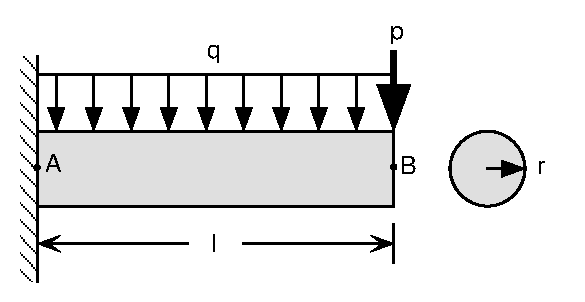
\includegraphics[clip=true]{beam.eps}
 \end{center}
\caption{Cantilever Beam}
\label{fig.beam}
\end{figure}
\begin{verbatim}
\begin{figure}[!htbp]
 \begin{center}
  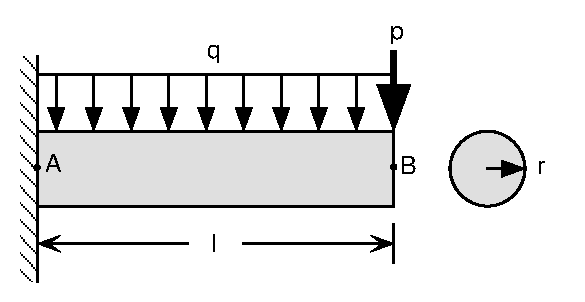
\includegraphics[clip=true]{beam.eps}
 \end{center}
\caption{Cantilever Beam}
\label{fig.beam}
\end{figure}
\end{verbatim}
Note the \enviro{figure} environment, which provides for captioning, and \enviro{center} environment for positioning the figure.

Figures can also be pasted in by hand if you leave room for them.
The following commands will leave a vertical space of 2.5 inches with a caption.
\begin{verbatim}
\begin{figure}
\vspace{2.5in}
\caption{Caption for Figure and for List of Figures - up to 300 chars}
\end{figure}
\end{verbatim}
%======================================================================
\section{Tables}
%======================================================================
Tables are easy to generate in \LaTeX .
Simple tables can be produced with the \enviro{tabbing} environment, as seen
in Section~\ref{ssec.fontfam}.
The source for that table is as follows:
\begin{verbatim}
\begin{tabbing}
mmmmm\=mmmmmmmmmmmmm\= \kill
\>\textbf{Command} \>\textbf{Description} \\
\>\cmmd{textrm} \>roman family \\
\>\cmmd{textsf} \>sans serif family \\
\>\cmmd{texttt} \>typewriter family \\
\>\cmmd{textbf} \>bold series \\
\>\cmmd{textmd} \>medium series \\
\>\cmmd{textit} \>italic shape \\
\>\cmmd{textsl} \>slanted shape \\
\>\cmmd{textup} \>upright shape (default)
\end{tabbing}
\end{verbatim}
Tabs are set with \cmmd{=}.
The \cmmd{kill} command cancels the line after the tabs are set. 
The \cmmd{>} moves to the next set tab stop.

The \enviro{table} and \enviro{tabular} environments can be used to produce captioned and bordered tables.
The following Table~\ref{tab.results} provides an example.
\begin{table}[!htbp]
\begin{center}
\begin{tabular}{|c||cc|cc|}
\hline
& \multicolumn{2}{c|}{ {\textbf CCP Rel. Indices} } 
& \multicolumn{2}{c|}{ {\textbf FORM Rel. Indices} } \\ 
\cline{2-5}
& $\beta_{MVFO}$ & $\beta_{MVMS}$ & $\beta_{FOSM}$ & $\beta_{FO}$ \\
\hline \hline
$\left\{ r^\star \, | \, \beta_1 \geq 3.719 \right\}$
& 1.347\dag & 1.348\dag & 1.325 & 1.175 \\
Rel. Error & +14.6\% & +14.7\% & +12.8\% & --- \\
%($\beta_2$) & (6.670) & (6.540) & (3.022) & (1.763) \\
\hline
$\left\{ r^\star \, | \, \beta_2 \geq 3.092 \right\}$
& 1.213 & 1.220 & 1.337\dag & 1.290\dag \\
Rel. Error & -6.0\% & -5.4\% & +3.6\% & --- \\
%($\beta_1$) & (3.222) & (3.251) & (3.755) & (4.742) \\
\hline
\end{tabular}
\begin{tabular}{l}
\footnotesize % smaller text in this environment only
\dag Active constraint when both are considered in the design 
optimization.
\end{tabular}
\end{center}
\caption{Minimum Beam Radius Using Four Reliability Indices}
\label{tab.results}
\end{table}
\begin{verbatim}
\begin{table}[!htbp]
\begin{center}
\begin{tabular}{|c||cc|cc|}
\hline
& \multicolumn{2}{c|}{ {\textbf CCP Rel. Indices} }
& \multicolumn{2}{c|}{ {\textbf FORM Rel. Indices} } \\
\cline{2-5}
& $\beta_{MVFO}$ & $\beta_{MVMS}$ & $\beta_{FOSM}$ & $\beta_{FO}$ \\
\hline \hline
$\left\{ r^\star \, | \, \beta_1 \geq 3.719 \right\}$
& 1.347\dag & 1.348\dag & 1.325 & 1.175 \\
Rel. Error & +14.6\% & +14.7\% & +12.8\% & --- \\
%($\beta_2$) & (6.670) & (6.540) & (3.022) & (1.763) \\
\hline
$\left\{ r^\star \, | \, \beta_2 \geq 3.092 \right\}$
& 1.213 & 1.220 & 1.337\dag & 1.290\dag \\
Rel. Error & -6.0\% & -5.4\% & +3.6\% & --- \\
%($\beta_1$) & (3.222) & (3.251) & (3.755) & (4.742) \\
\hline
\end{tabular}
\begin{tabular}{l}
\footnotesize % small text inside this environment only
\dag Active constraint when both are considered in the design 
optimization.
\end{tabular}
\end{center}
\caption{Minimum Beam Radius Using Four Reliability Indices}
\label{tab.results}
\end{table}
\end{verbatim}
Note that a second \enviro{tabular} environment was used to produce a footnote under the table.
A \enviro{minipage} environment around the table could also have been used.
%======================================================================
\section{Math Structures}
%======================================================================
\LaTeX\ uses an intuitive language for formatting mathematics.
Some examples of the main math environments will give the idea.
%----------------------------------------------------------------------
\subsection{In-Line Math}
%----------------------------------------------------------------------
In-line math may be inserted between \cmmd{(} and \cmmd{)}, or \$ and \$ (the latter form being preferred since it is not fragile).
For example,
\begin{verbatim}
\rv{A} is a random matrix of size $m \times n$ ($m < n$).
\end{verbatim}
produces ``\rv{A} is a random matrix of size $m \times n$ ($m < n$)''.
%----------------------------------------------------------------------
\subsection{Displayed Formulae}
%----------------------------------------------------------------------
Math may also be displayed (set apart from the text) with the \enviro{displaymath}, or between the short-cut commands \cmmd{[} and \cmmd{]}.
For example,
\begin{verbatim}
\begin{displaymath}
\beta \equiv \Phi^{-1}( \gamma )
\end{displaymath}
\end{verbatim}
produces
\begin{displaymath}
\beta \equiv \Phi^{-1}( \gamma )
\end{displaymath}
%----------------------------------------------------------------------
\subsection{Numbered Equations}
%----------------------------------------------------------------------
Numbered equations are produced inside the \enviro{equation} environment.
For example,
\begin{verbatim}
\begin{equation}
\label{eqn.gradbetaFO}
\nabla_D \beta_{FO} = \nabla_D \beta_{FOSM} =
\frac{ \nabla_{D} g_{i} (U^{\star} }{ \| \nabla_{U} g_{i} 
(U^{\star}) \| }
\end{equation}
\end{verbatim}
produces
\begin{equation}
\label{eqn.gradbetaFO}
\nabla_D \beta_{FO} = \nabla_D \beta_{FOSM} =
\frac{ \nabla_{D} g_{i} (U^{\star}) }{ \| \nabla_{U} g_{i} 
(U^{\star}) \| }
\end{equation}
%----------------------------------------------------------------------
\subsection{Equation Arrays}
%----------------------------------------------------------------------
The \enviro{eqnarray} produces equation arrays, which are structures for multi-line formulae.
Each line is given a number, unless this is suppressed with \cmmd{nonumber} command.
Numbering may be suppressed for the whole environment if the \enviro{eqnarray*} form of the environment command is used.
For example,
\begin{eqnarray}
  {\mathrm optimize} & \rv{C}^{T} X  \label{eqn.lpobjective} \\
  {\mathrm subject \: to} & \rv{A} X \leq  \rv{B} 
  \label{eqn.lpconstraints}
\end{eqnarray}
is produced by 
\begin{verbatim}
\begin{eqnarray}
  {\mathrm optimize} & \rv{C}^{T} X  \label{eqn.lpobjective} \\
  {\mathrm subject \: to} & \rv{A} X \leq  \rv{B} 
  \label{eqn.lpconstraints}
\end{eqnarray}
\end{verbatim}
Note that since each line is numbered, each may be given a label.
The \enviro{eqnarray} environment allows three columns, aligned on the \& symbols.
%----------------------------------------------------------------------
\subsection{Math Fonts}
\label{ssec.mathfonts}
%----------------------------------------------------------------------
Just as there are different type styles available in text mode, there are also math mode type styles, summarized below.
\begin{tabbing}
mmmmm\=mmmmmmmmmmmmm\= \kill
\>\textbf{Command} \>\textbf{Description} \\
\>\cmmd{mathrm} \>$\mathrm{roman}$ family\\
\>\cmmd{mathsf} \>$\mathsf{sans \: serif}$ family\\
\>\cmmd{mathtt} \>$\mathtt{typewriter}$ family\\
\>\cmmd{mathbf} \>$\mathbf{bold}$ series\\
\>\cmmd{mathit} \>$\mathit{italic}$ shape\\
\>\cmmd{mathcal} \>$\mathcal{CALIGRAPHIC}$ shape (upper case only)
\end{tabbing}
These commands only change the style of letters, numbers, and uppercase Greek letters, not other math symbols.
%======================================================================
\section{Appendices}
%======================================================================
Appendices may be included by simply adding an \cmmd{appendix} command in your master document.
All logical structures (chapters, sections, \etc) which appear below that point will then be ``numbered'' with letters.
%======================================================================
\section{Bibliography}
%======================================================================
A bibliography can be created two ways in \LaTeX , ``by hand'' or by using the \program{bibtex} program.
Once the bibliography items have been created by one of these methods, they are referred to in the \LaTeX\ source files with the \cmmd{cite} command. 
For example,
\begin{verbatim}
\LaTeX\ is a set of macros by Leslie Lamport \cite{lamport.book}.
\end{verbatim}
%----------------------------------------------------------------------
\subsection{``By-Hand'' Method}
%----------------------------------------------------------------------
In the ``End Material'' section of your master source file include your bibliography list, which you must format yourself. 
For example,
\begin{verbatim}
\begin{thebibliography}{9}
\bibitem{jungle.book} Jungle, George 
        {\em Watch Out for That Tree}
        Toronto: University of Toronto Press, 1986.
\bibitem{cliches.book} Smith, J.\ Henry.  
        {\em Cliches and Platitudes for Every Occasion}
        Ottawa: Political Press, 1996
\end{thebibliography}
\end{verbatim}
The second argument in the \cmmd{begin\{thebibliography\}\{9\}} is a number greater than the number of references to be formatted.  
The label parameter in the \cmmd{bibitem} command is used in the \cmmd{cite} command.
%----------------------------------------------------------------------
\subsection{Using BibTeX}
%----------------------------------------------------------------------
It is often easier to keep your bibliographic data together in bibliographic databases.
The \program{bibtex} program works with \LaTeX\ by gathering cited references from specified databases (text files with extension \exten{bib}, called \exten{BIB} files) and formatting the bibliography according to a desired style.
This method is much easier than doing the formatting ``by hand''.
If you create your own \exten{BIB} files, put them in the same directory as your \LaTeX\ source files, or set \program{latex}'s BIBINPUTS environment variable (under Unix) to the correct path.

The \program{bibtex} program is run after the \program{latex} program since it uses the \exten{AUX} files produced by \program{latex}.
The style and position of the bibliography in the final document is indicated by inserting the \cmmd{bibstyle} and \cmmd{bibliography} commands in the master \LaTeX\ source file.
The bibliography section by default does not appear in the Table of Contents. 
Adding it just requires manual editing of the file with extension \exten{TOC}, produced by \program{latex}, followed by a final run of \program{latex}.

The bibliography is formated according to the specified \cmmd{bibstyle} for each type of reference given: books, journals, collections, \etc .
The \texttt{bib} file used for this document is given below.
\begin{verbatim}
% Bibliography of key references for "LaTeX for Thesis 
% and Large Documents"
% For use with BibTeX

@book{goossens.book,
        author =	"Michel Goossens and Frank Mittelbach and 
        		 Alexander Samarin",
        title =		"The \LaTeX\ Companion",
        year = 		"1994",
        publisher =	"Addison-Wesley",
        address = 	"Reading, Massachusetts"
}

@book{knuth.book,
        author =        "Donald Knuth",
        title =         "The \TeX book",
        year =          "1986",
        publisher =     "Addison-Wesley",
        address =       "Reading, Massachusetts"
}

@book{lamport.book,
        author =        "Leslie Lamport",
        title =         "\LaTeX\ --- A Document Preparation System",
        edition =       "Second",
        year = 		"1994",
        publisher = 	"Addison-Wesley",
        address =       "Reading, Massachusetts"
}
\end{verbatim}
%======================================================================
\section{Glossary} 
%======================================================================
There is no specific \LaTeX\ command for creating a glossary.
However, one can easily be produced with the \enviro{description} environment, as shown in Appendix~\ref{chap.glossary}. 

The \program{makeindex} program can also be used to create a Glossary automatically, if terms are defined in specific places in your document.
%======================================================================
\section{Index}
%======================================================================
An index can be created two ways in \LaTeX , ``by hand'' or by using the \program{makeindex} program.
%----------------------------------------------------------------------
\subsection{``By-Hand'' Method}
%----------------------------------------------------------------------
In the ``End Material'' section of your master source file include your index with the \enviro{theindex} environment, then format it yourself.
For example,
\begin{verbatim}
\begin{theindex}
\item \LaTeX 3
   \subitem program, 4
      \subsubitem running, 5
\indexspace
\item \program{bibtex} 12
   \subitem running, 13
\end{theindex}
\end{verbatim}
%----------------------------------------------------------------------
\subsection{Using MakeIndex}
%----------------------------------------------------------------------
Use of the \program{makeindex} progam is recommended as a significant improvement over producing an index by hand.
If using \program{makeindex}, indexed items are
referred to in the \LaTeX\ source files with the \cmmd{index} command.
For example,
\begin{verbatim}
\LaTeX\index{\LaTeX} is a set of macros ...
\end{verbatim}
There are several other variations of the \cmmd{index} command which assist in formatting and ordering the index items.

To use \program{makeindex}, put a \verb=\usepackage{makeidx}= command in the preamble of your master source file.
If the command \cmmd{makeindex} also exists in the preamble of your master source file, \LaTeX\ will produce an \exten{IDX} file which is processed by \program{makeindex} to produce the final \exten{IND} file.
The \cmmd{printindex} command is placed in the master source document where you want the index to go in the end material.
Running \program{latex} again will place the index in the output \exten{DVI} file.
Note also that the index does not by default appear in the Table of Contents.
It must be added by hand, as was done for the Bibliography.
 %"Example \LaTeX\ Commands for Large Documents" 
\chapter{Processing Your \LaTeX\ Source Files Under Unix}
\markright{Processing Your \LaTeX\ Source Files Under Unix} % new right header
%======================================================================
\section{Running \program{latex}}
%======================================================================
The \program{latex}\index{\LaTeX!running} program is executed on your master source file:
\begin{verbatim}
% latex master  (for a source file called master.tex)
\end{verbatim}
If you are using \program{bibtex} or \program{makeindex}, run these next:
\begin{verbatim}
% bibtex master  (for source file master.tex)
% makeindex master
\end{verbatim}
Run \program{latex} at least twice more to process all the labels and references.
The resulting typeset document is in a file called \verb=master.dvi=.
%======================================================================
\section{Syntax Checking}
%======================================================================
\index{\LaTeX!syntax checking}
You will notice that \LaTeX\ doesn't always give the most instructive error messages.
It is useful to use a utility called \program{lacheck} to check for syntax errors before using the \program{latex} program.
\begin{verbatim}
% lacheck *.tex  (check all your .tex files)
\end{verbatim}
%======================================================================
\section{Spell Checking}
%======================================================================
The Unix \program{correct} program is useful for checking spelling.
\begin{verbatim}
% correct -l master.tex  (-l option filters LaTeX commands)
\end{verbatim}
%======================================================================
\section{Previewing the Typeset Document}
%======================================================================
\index{\LaTeX!previewing}
The typeset document is in a \exten{DVI} file, \eg\ \verb=master.dvi=.
This file may be previewed using either the \program{xdvi} or \program{ghostview} programs.
It is a good idea to view your document frequently as you develop it.
It's easier to debug your \LaTeX\ source files as you work, rather than all at once.

To use \program{xdvi}, run it on the \exten{DVI} file.
\begin{verbatim}
% xdvi master.dvi  (for source file master.tex)
\end{verbatim}

To use \program{ghostview}, process the \exten{DVI} file with \program{dvips} to produce a PostScript file then use \program{ghostview} to view it.
\begin{verbatim}
% dvips master.dvi > master.ps   (for source file master.tex)
% ghostview master.ps
\end{verbatim}
%======================================================================
\section{Printing}
%======================================================================
Once you are satisfied with the final document you may print it using the \program{lpr} command.
\begin{verbatim}
% lpr -Plw -Fd master.dvi  (for source file master.tex)
OR ...
% lpr -Plw master.ps
\end{verbatim}
You may also print directly from \program{ghostview}.

If you wish to print only some of the pages of your document, \program{ghostview} will let you do that.
Alternatively, you can use the \program{dviselect} to print selected pages from a \exten{DVI} file, for example
\begin{verbatim}
% dviselect -i master.dvi -o somepages.dvi 5-12 13 17
\end{verbatim}
will place pages 5--12, 13, and 17 in a new \exten{DVI} file called ``somepages'', which then must be sent to the printer as outlined above.
%======================================================================
\section{Creating Portable Document Format (PDF)}
%======================================================================
If you wish to create an electronic version of your document,
rather than a paper version, a good choice is to create a PDF file, and \LaTeX\ provides utilities for doing so.

PDF documents allow enriched features, such as hyperlinks. The \program{hyperref} package can be included in your master source file to automate internal hyperlinking in your document, as well as other features.

One important point to consider when creating a PDF file is the use of scalable fonts and graphics, to a avoid a ``jaggy'' appearance (loss of resolution) when you magnify a page. 

This course demonstrates the inclusion of Encapsulated Postscript (EPS) files as figures. These are created by ``printing to file'' through a Postscript printer driver from a drawing or plotting application. EPS files are scalable graphics, so work well when creating PDF.

By default, \LaTeX\ uses its own bit-mapped fonts (the Computer Modern set) when a printed document is produced. These bit-mapped fonts create blurry, ``jaggy'' results when converted to PDF. The way around this is to use the Postscript fonts made available under \LaTeXe. Alternative Postscript fonts can be specified in the master document preamble by including font packages. There are also Postscript versions of the default Computer Modern font sets. To make sure the PS versions of the default Computer Modern fonts are used when creating a PS file via \program{dvips}, use the \texttt{-Ppdf} option (see below).

There are two methods to create a PDF file. 
\begin{enumerate}
\item Create PDF directly from your \texttt{.tex} source filesby using the \program{pdflatex} program instead of \program{latex}.
\item Create a Postscript file then use \program{Adobe Acrobat} ``distiller'' or \program{Ghostview/GSView} to create the PDF file.
\begin{verbatim}
% dvips -Ppdf master.dvi > master.ps   (note use of -Ppdf option)
\end{verbatim}
\end{enumerate}
 %"Processing the Source File"
%----------------------------------------------------------------------
% END MATERIAL
%----------------------------------------------------------------------
%###################################
%## Edit this part
%###################################
% Appendices
\appendix
% Designate with \appendix declaration which just changes numbering style 
% from here on
%\include{useful_pkgs} %"Some Useful \LaTeX2e Packages"
% An appendix
%======================================================================
\chapter{Sources of Information and Help}
\markright{Sources of Information and Help}
%======================================================================
The best source of information about \LaTeX\ is the two books mentioned in this course \cite{lamport.book,goossens.book}.
Another excellent resource is the UseNet newsgroup \verb=comp.text.tex=.
A frequently-asked-questions (FAQ) list is also maintained by this news group.
You might also search the World Wide Web for ``LaTeX'' for other sources of help.
 %"Sources of Information and Help"

% Glossary
% You could use a \begin{description} ... \end{description} for this
\chapter{Glossary of Terms}
\markright{Glossary of Terms} % new right header
\label{chap.glossary}
%======================================================================
\begin{description}
% - - - - - - - - - - - - - - - - - - - - - - - - - - - - - - - - - - -
\item[left-to-right (LR) mode] Like paragraph mode, but no line breaks are inserted. The \cmmd{mbox} command is processed in LR mode.
% - - - - - - - - - - - - - - - - - - - - - - - - - - - - - - - - - - -
\item[math mode] The mode for typesetting mathematics. 
Math mode is indicated in in-line text between \cmmd{(}  \cmmd{)} commands or pairs of \$ symbols.
The \enviro{equation} and similar environments also work in math mode.
(Note that matched \$ s within these environments toggles back to paragraph mode.)
% - - - - - - - - - - - - - - - - - - - - - - - - - - - - - - - - - - -
\item[mode] One of three typesetting modes of \LaTeX : paragraph mode, math mode, left-to-right (LR) mode.
% - - - - - - - - - - - - - - - - - - - - - - - - - - - - - - - - - - -
\item[paragraph mode] The mode for processing ordinary text.
% - - - - - - - - - - - - - - - - - - - - - - - - - - - - - - - - - - -
\item[preamble] The material in a \LaTeX\ source file before the 
\verb=\begin{document}= command. 
Used to set the \cmmd{documentclass}, packages (\enviro{usepackage}), and other formatting commands.
% - - - - - - - - - - - - - - - - - - - - - - - - - - - - - - - - - - -
\end{description}


% Bibliography 
% If done using the BibTeX program, use
\bibliographystyle{plain} % sorted alphabetically, labeled with numbers
\bibliography{bibliography/keylatex} % names file keylatex.bib as my bibliography file 
% OR, do it "by hand" inside a "thebibliography" enivironment

% Index 
% Put a \makeindex command in the Preamble if you use MakeIndex program
% and put 
\printindex % here
% OR, do it "by hand" inside \begin{theindex} ... \end{theindex}
%----------------------------------------------------------------------
\end{document}
%======================================================================
\end{verbatim}
\end{small}
